% UCL Thesis LaTeX Template
%  (c) Ian Kirker, 2014
% 
% This is a template/skeleton for PhD/MPhil/MRes theses.
%
% It uses a rather split-up file structure because this tends to
%  work well for large, complex documents.
% We suggest using one file per chapter, but you may wish to use more
%  or fewer separate files than that.
% We've also separated out various bits of configuration into their
%  own files, to keep everything neat.
% Note that the \input command just streams in whatever file you give
%  it, while the \include command adds a page break, and does some
%  extra organisation to make compilation faster. Note that you can't
%  use \include inside an \include-d file.
% We suggest using \input for settings and configuration files that
%  you always want to use, and \include for each section of content.
% If you do that, it also means you can use the \includeonly statement
%  to only compile up the section you're currently interested in.
% You might also want to put figures into their own files to be \input.

% For more information on \input and \include, see:
%  http://tex.stackexchange.com/questions/246/when-should-i-use-input-vs-include


% Formatting and binding rules for theses are here: 
%  https://www.ucl.ac.uk/students/exams-and-assessments/research-assessments/format-bind-and-submit-your-thesis-general-guidance

% This package goes first and foremost, because it checks all 
%  your syntax for mistakes and some old-fashioned LaTeX commands.
% Note that normally you should load your documentclass before 
%  packages, because some packages change behaviour based on
%  your document settings.
% Also, for those confused by the RequirePackage here vs usepackage
%  elsewhere, usepackage cannot be used before the documentclass
%  command, while RequirePackage can. That's the only functional
%  difference as far as I'm aware.
\RequirePackage[l2tabu, orthodox]{nag}

% ------ Main document class specification ------
% The draft option here prevents images being inserted,
%  and adds chunky black bars to boxes that are exceeding 
%  the page width (to show that they are).
% The oneside option can optionally be replaced by twoside if
%  you intend to print double-sided. Note that this is
%  *specifically permitted* by the UCL thesis formatting
%  guidelines.
%
% Valid options in terms of type are:
%  phd
%  mres
%  mphil
%\documentclass[12pt,phd,draft,a4paper,oneside]{ucl_thesis}
\documentclass[12pt,mpa,a4paper,oneside]{ucl_thesis}%,scribble


% Package configuration:
%  LaTeX uses "packages" to add extra commands and features.
%  There are quite a few useful ones, so we've put them in a 
%   separate file.
% -------- Packages --------

% This package just gives you a quick way to dump in some sample text.
% You can remove it -- it's just here for the examples.
\usepackage{blindtext}

% This package means empty pages (pages with no text) won't get stuff
%  like chapter names at the top of the page. It's mostly cosmetic.
\usepackage{emptypage}

% The graphicx package adds the \includegraphics command,
%  which is your basic command for adding a picture.
\usepackage{graphicx}

% The float package improves LaTeX's handling of floats,
%  and also adds the option to *force* LaTeX to put the float
%  HERE, with the [H] option to the float environment.
\usepackage{float}

% The amsmath package enhances the various ways of including
%  maths, including adding the align environment for aligned
%  equations.
\usepackage{amsmath}

% Use these two packages together -- they define symbols
%  for e.g. units that you can use in both text and math mode.
\usepackage{gensymb}
\usepackage{textcomp}
% You may also want the units package for making little
%  fractions for unit specifications.
%\usepackage{units}


% The setspace package lets you use 1.5-sized or double line spacing.
\usepackage{setspace}
\setstretch{1.5}

% That just does body text -- if you want to expand *everything*,
%  including footnotes and tables, use this instead:
%\renewcommand{\baselinestretch}{1.5}


% PGFPlots is either a really clunky or really good way to add graphs
%  into your document, depending on your point of view.
% There's waaaaay too much information on using this to cover here,
%  so, you might want to start here:
%   http://pgfplots.sourceforge.net/
%  or here:
%   http://pgfplots.sourceforge.net/pgfplots.pdf
%\usepackage{pgfplots}
%\pgfplotsset{compat=1.3} % <- this fixed axis labels in the version I was using

% PGFPlotsTable can help you make tables a little more easily than
%  usual in LaTeX.
% If you're going to have to paste data in a lot, I'd suggest using it.
%  You might want to start with the manual, here:
%  http://pgfplots.sourceforge.net/pgfplotstable.pdf
%\usepackage{pgfplotstable}

% These settings are also recommended for using with pgfplotstable.
%\pgfplotstableset{
%	% these columns/<colname>/.style={<options>} things define a style
%	% which applies to <colname> only.
%	empty cells with={--}, % replace empty cells with '--'
%	every head row/.style={before row=\toprule,after row=\midrule},
%	every last row/.style={after row=\bottomrule}
%}


% The mhchem package provides chemistry formula typesetting commands
%  e.g. \ce{H2O}
%\usepackage[version=3]{mhchem}

% And the chemfig package gives a weird command for adding Lewis 
%  diagrams, for e.g. organic molecules
%\usepackage{chemfig}

% The linenumbers command from the lineno package adds line numbers
%  alongside your text that can be useful for discussing edits 
%  in drafts.
% Remove or comment out the command for proper versions.
%\usepackage[modulo]{lineno}
% \linenumbers 


% Alternatively, you can use the ifdraft package to let you add
%  commands that will only be used in draft versions
%\usepackage{ifdraft}

% For example, the following adds a watermark if the draft mode is on.
%\ifdraft{
%  \usepackage{draftwatermark}
%  \SetWatermarkText{\shortstack{\textsc{Draft Mode}\\ \strut \\ \strut \\ \strut}}
%  \SetWatermarkScale{0.5}
%  \SetWatermarkAngle{90}
%}


% The multirow package adds the option to make cells span 
%  rows in tables.
\usepackage{multirow}
\usepackage{tabularx}
\usepackage{array}
\newcolumntype{L}[1]{>{\raggedright\arraybackslash}p{#1-2\tabcolsep}}
\newcolumntype{B}[1]{>{\raggedright\arraybackslash}b{#1-2\tabcolsep}}
\setlength\extrarowheight{1ex} % make the tables look less cramped

% Subfig allows you to create figures within figures, to, for example,
%  make a single figure with 4 individually labeled and referenceable
%  sub-figures.
% It's quite fiddly to use, so check the documentation.
%\usepackage{subfig}

% makeidx enables an index to be inserted
\usepackage{makeidx}
\usepackage{soul}

%----------------------------------------------------------------------------------------
%	izzys colours
%----------------------------------------------------------------------------------------
\usepackage[pdftex,dvipsnames,table]{xcolor}  % Coloured text etc.
\definecolor{izpink}{rgb}{1,.9,95}
\definecolor{izgreen}{rgb}{0,0.5,0}
\definecolor{citecolor}{rgb}{0.1,0.4,0.1}
\definecolor{orangelinks}{RGB}{210, 60, 4}
\definecolor{izorange}{RGB}{204, 51, 0}
\definecolor{headblue}{rgb}{.7,.81,0.9}
\newcommand{\pinkcell}{\cellcolor{izpink}}
\newcommand{\linkcolor}{izgreen}


%----------------------------------------------------------------------------------------
% Izzy's prefered reference package is biblatex
%----------------------------------------------------------------------------------------
% The natbib package allows book-type citations commonly used in
%  longer works, and less commonly in science articles (IME).
% e.g. (Saucer et al., 1993) rather than [1]
% More details are here: http://merkel.zoneo.net/Latex/natbib.php
%\usepackage{natbib}

% The bibentry package (along with the \nobibliography* command)
%  allows putting full reference lines inline.
%  See: 
%   http://tex.stackexchange.com/questions/2905/how-can-i-list-references-from-bibtex-file-in-line-with-commentary
%\usepackage{bibentry} 
\usepackage[utf8]{inputenc}
\usepackage[english]{babel}
\usepackage{csquotes}
\usepackage[uniquename=false,
date=year,
maxbibnames=2,%9
maxcitenames=2,
uniquelist=false,
backend=biber,
language=british,
hyperref=true,
%backref=true,
%style=phys, sorting=none
%style=geschichtsfrkl
%style=numeric-comp,sorting=none
% --- Superscript numbers in citation:
%style=numeric, sorting=none,autocite=superscript % set document option to endnotes
%style=authoryear % set document option to authoryear
natbib=true,%url=false,%eprint=false,
style=\bibtype, sorting=\bibsort, autocite=\bibauto
]{biblatex}
\renewcommand*{\citesetup}{%
  \color{citecolor}
  \biburlsetup
  \frenchspacing}

% this renders et al. in italics:
\renewbibmacro*{name:andothers}{% Based on name:andothers from biblatex.def
  \ifboolexpr{
    test {\ifnumequal{\value{listcount}}{\value{liststop}}}
    and
    test \ifmorenames
  }
    {\ifnumgreater{\value{liststop}}{1}
       {\finalandcomma}
       {}%
     \andothersdelim\bibstring[\emph]{andothers}}
    {}}
% The isorot package allows you to put things sideways 
%  (or indeed, at any angle) on a page.
% This can be useful for wide graphs or other figures.
%\usepackage{isorot}

% The caption package adds more options for caption formatting.
% This set-up makes hanging labels, makes the caption text smaller
%  than the body text, and makes the label bold.
% Highly recommended.
\usepackage[format=hang,font=small,labelfont=bf]{caption}

% If you're getting into defining your own commands, you might want
%  to check out the etoolbox package -- it defines a few commands
%  that can make it easier to make commands robust.
\usepackage{etoolbox}

% The microtype package adds `micro-typographic extensions' which
% generally makes text more readable and hyphenation less likely.
\usepackage{microtype}

\usepackage{ifthen}
%\usepackage{tocbibind} %don't use this, it forces Contents to be in the toc

%----------------------------------------------------------------------------------------
% To Do notes 
%----------------------------------------------------------------------------------------
\usepackage{nameref}
\makeatletter
\newcommand*{\currentname}{\@currentlabelname}
\makeatother
% nice example of using todonotes package: https://tex.stackexchange.com/questions/9796/how-to-add-todo-notes
\usepackage{xargs}                      % Use more than one optional parameter in a new commands
\usepackage[colorinlistoftodos,prependcaption,textsize=tiny]{todonotes}
\newcommandx{\unsure}[2][1=]{\todo[linecolor=red,backgroundcolor=red!25,bordercolor=red,#1]{#2}}
\newcommandx{\change}[2][1=]{\todo[linecolor=blue,backgroundcolor=blue!25,bordercolor=blue,#1]{#2}}
\newcommandx{\info}[2][1=]{\todo[linecolor=OliveGreen,backgroundcolor=OliveGreen!25,bordercolor=OliveGreen,#1]{#2}}
\newcommandx{\improvement}[2][1=]{\todo[linecolor=Plum,backgroundcolor=Plum!25,bordercolor=Plum,#1]{#2}}% in: \textbf{\currentname}


%----------------------------------------------------------------------------------------
% Izzy's commands
%----------------------------------------------------------------------------------------
% this one enables highlighting of the quotes from a particular participant (intended for participants to individually review their contribution)
\newcommand{\hp}{p00}
\newcommand{\tquote}[3]{%add a third argument for the quote ID
    \ifthenelse{\equal{#2}{\hp}}{%
        \definecolor{thighlightc}{rgb}{1,1,.2}}{%
        \definecolor{thighlightc}{rgb}{1,1,1}%
    }%
    \sethlcolor{thighlightc}%
    \hl{``\emph{#1}''}%
}
\newcommand{\tref}[2]{%
    \ifthenelse{\equal{#2}{\hp}}{%
        \definecolor{thighlightc}{rgb}{1,1,.2}}{%
        \definecolor{thighlightc}{rgb}{1,1,1}%
    }%
    \sethlcolor{thighlightc}%
    \hl{#1}%
}

% izquote
\newcommand{\izquote}[2]{
    \parbox{.8\textwidth}{\raggedright\emph{#1}}\\[5mm]
    \parbox{.8\textwidth}{\raggedleft #2}
}


% make ISM factors have unique font
%\DeclareTextFontCommand{\ismfont}{\textsc}
\newcommand{\ismfont}[1]{\textsc{#1}} %change this if you want to change the font
\newcommand{\ismiv}{\ismfont{Values, Beliefs and Attitudes}}
\newcommand{\ismic}{\ismfont{Costs and Benefits}}
\newcommand{\ismie}{\ismfont{Emotions}}
\newcommand{\ismia}{\ismfont{Agency}}
\newcommand{\ismis}{\ismfont{Skills}}
\newcommand{\ismih}{\ismfont{Habit}}
\newcommand{\ismso}{\ismfont{Opinion leaders}}
\newcommand{\ismsi}{\ismfont{Institutions}}
\newcommand{\ismsn}{\ismfont{Norms}}
\newcommand{\ismsr}{\ismfont{Roles and Identities}}
\newcommand{\ismst}{\ismfont{Tastes}}
\newcommand{\ismsm}{\ismfont{Meanings}}
\newcommand{\ismsnr}{\ismfont{Networks and Relationships}}
\newcommand{\ismmr}{\ismfont{Rules and Regulations}}
\newcommand{\ismmt}{\ismfont{Technologies}}
\newcommand{\ismmi}{\ismfont{Infrastructure}}
\newcommand{\ismmo}{\ismfont{Objects}}
\newcommand{\ismmts}{\ismfont{Times and Schedules}}


\newcommand{\scip}{Governance System}
\newcommand{\know}{Knowledge System}
\newcommand{\inte}{Intra/Interpersonal System}
\newcommand{\valu}{Values, Beliefs and Attitudes}
\newcommand{\agen}{Agency and Effort}
\newcommand{\pers}{Perspectives}
\newcommand{\opin}{Opinion leaders}
\newcommand{\netw}{Networks and Relationships}
\newcommand{\skil}{Knowledge and Skills}
\newcommand{\tech}{Techniques}
\newcommand{\fram}{Frames}
\newcommand{\obje}{Objects}
\newcommand{\poli}{Policy Landscape}
\newcommand{\inst}{Institutions}
\newcommand{\infr}{Infrastructure}
\newcommand{\even}{Political Events and Cycles}
\newcommand{\role}{Roles and Identities}
\newcommand{\emot}{Emotions}

\newcommand{\skiscip}{\scip} %ss
\newcommand{\skiknow}{\know} %kk
\newcommand{\skiinte}{\inte} %ii
\newcommand{\skivalu}{\ismfont{\valu}} %iv
\newcommand{\skiagen}{\ismfont{\agen}} %ia
\newcommand{\skipers}{\ismfont{\pers}} %ip
\newcommand{\skiopin}{\ismfont{\opin}} %io
\newcommand{\skinetw}{\ismfont{\netw}} %in
\newcommand{\skiskil}{\ismfont{\skil}} %kk
\newcommand{\skitech}{\ismfont{\tech}} %kt
\newcommand{\skifram}{\ismfont{\fram}} %kf
\newcommand{\skiobje}{\ismfont{\obje}} %ko
\newcommand{\skipoli}{\ismfont{\poli}} %sp
\newcommand{\skiinst}{\ismfont{\inst}} %si
\newcommand{\skiinfr}{\ismfont{\infr}} %sif
\newcommand{\skieven}{\ismfont{\even}} %se
\newcommand{\skirole}{\ismfont{\role}} % r
\newcommand{\skiemot}{\ismfont{\emot}} % e

\newcommand{\titscip}{\scip}
\newcommand{\titknow}{\know}
\newcommand{\titinte}{\inte}
\newcommand{\titvalu}{\valu}
\newcommand{\titagen}{\agen}
\newcommand{\titpers}{\pers}
\newcommand{\titopin}{\opin}
\newcommand{\titnetw}{\netw}
\newcommand{\titskil}{\skil}
\newcommand{\tittech}{\tech}
\newcommand{\titfram}{\fram}
\newcommand{\titobje}{\obje}
\newcommand{\titpoli}{\poli}
\newcommand{\titinst}{\inst}
\newcommand{\titinfr}{\infr}
\newcommand{\titeven}{\even}
\newcommand{\titrole}{\role}
\newcommand{\titemot}{\emot}
%%%%%%%%%%%%%%%%%%%%%%%%%%%%%%%%%%%%%%%%%
%% GLOSSARY IS IN LinksAndMetadata.tex %%
%%%%%%%%%%%%%%%%%%%%%%%%%%%%%%%%%%%%%%%%%


% Sets up links within your document, for e.g. contents page entries
%  and references, and also PDF metadata.
% You should edit this!
%%
%% This file uses the hyperref package to make your thesis have metadata embedded in the PDF, 
%%  and also adds links to be able to click on references and contents page entries to go to 
%%  the pages.
%%

% Some hacks are necessary to make bibentry and hyperref play nicely.
% See: http://tex.stackexchange.com/questions/65348/clash-between-bibentry-and-hyperref-with-bibstyle-elsart-harv
\usepackage{bibentry}
\makeatletter\let\saved@bibitem\@bibitem\makeatother
\usepackage[pdftex,hidelinks]{hyperref}
\makeatletter\let\@bibitem\saved@bibitem\makeatother
\makeatletter
\AtBeginDocument{
    \hypersetup{
        pdfsubject={Thesis Subject},
        pdfkeywords={Thesis Keywords},
        pdfauthor={Author},
        pdftitle={Title},
    }
}
\makeatother
    
%----------------------------------------------------------------------------------------
%	izzys hyperlinks
%----------------------------------------------------------------------------------------
\hypersetup{
    colorlinks=true,
    linkcolor=\linkcolor,%{[rgb]{0,0.5,0}},
    filecolor=blue,
    citecolor=\linkcolor,%{[rgb]{0,0.5,0}},
    urlcolor=\linkcolor,%{[rgb]{0,0.5,0}},
    pdftitle={Overleaf Example},
    pdfpagemode=UseOutlines%,FullScreen,
    }

\urlstyle{same}

% And then some settings in separate files.
\input{FloatSettings} % For things like figures and tables
%\input{BibSettings}   % For bibliographies

% These control how many number sections your subsections will take
%    e.g. Section 2.3.1.5.6.3
%  and how many of those will get put into the contents pages.
\setcounter{secnumdepth}{3}
\setcounter{tocdepth}{3}

\addbibresource{izzy.bib}
\addbibresource{izzy_2013_2021.bib}
\addbibresource{izzy_2022_2023.bib}
%\makenoidxglossaries
\makeglossaries
%\makeindex

\begin{document}
%\nobibliography*
% ^-- This is a dumb trick that works with the bibentry package to let
%  you put bibliography entries whereever you like.
% I used this to put references to papers a chapter's work was 
%  published in at the end of that chapter.
% For more information, see: http://stefaanlippens.net/bibentry

% If you haven't finished making your full BibTex file yet, you
%  might find this useful -- it'll just replace all your
%  citations with little superscript notes.
% Uncomment to use.
%\renewcommand{\cite}[1]{\emph{\textsuperscript{[#1]}}}

% At last, content! Remember filenames are case-sensitive and 
%  *must not* include spaces.
% I may change the way this is done in a future version, 
%  but given that some people needed it, if you need a different degree title 
%  (e.g. Master of Science, Master in Science, Master of Arts, etc)
%  uncomment the following 3 lines and set as appropriate (this *has* to be before \maketitle)
% \makeatletter
% \renewcommand {\@degree@string} {Master of Things}
% \makeatother

\title{Science at the climate policy interface}
\author{Isabel M J Sargent}
\department{Institute for Innovation and Public Purpose}

\maketitle

%%%%%%%% commented out more of preamble for now
\iffalse
\makedeclaration

\begin{abstract} % 300 word limit
My research is about stuff.

It begins with a study of some stuff, and then some other stuff and things.

There is a 300-word limit on your abstract.
\end{abstract}

\begin{impactstatement}

	UCL theses now have to include an impact statement. \textit{(I think for REF reasons?)} The following text is the description from the guide linked from the formatting and submission website of what that involves. (Link to the guide: {\scriptsize \url{http://www.grad.ucl.ac.uk/essinfo/docs/Impact-Statement-Guidance-Notes-for-Research-Students-and-Supervisors.pdf}})

\begin{quote}
The statement should describe, in no more than 500 words, how the expertise, knowledge, analysis,
discovery or insight presented in your thesis could be put to a beneficial use. Consider benefits both
inside and outside academia and the ways in which these benefits could be brought about.

The benefits inside academia could be to the discipline and future scholarship, research methods or
methodology, the curriculum; they might be within your research area and potentially within other
research areas.

The benefits outside academia could occur to commercial activity, social enterprise, professional
practice, clinical use, public health, public policy design, public service delivery, laws, public
discourse, culture, the quality of the environment or quality of life.

The impact could occur locally, regionally, nationally or internationally, to individuals, communities or
organisations and could be immediate or occur incrementally, in the context of a broader field of
research, over many years, decades or longer.

Impact could be brought about through disseminating outputs (either in scholarly journals or
elsewhere such as specialist or mainstream media), education, public engagement, translational
research, commercial and social enterprise activity, engaging with public policy makers and public
service delivery practitioners, influencing ministers, collaborating with academics and non-academics
etc.

Further information including a searchable list of hundreds of examples of UCL impact outside of
academia please see \url{https://www.ucl.ac.uk/impact/}. For thousands more examples, please see
\url{http://results.ref.ac.uk/Results/SelectUoa}.
\end{quote}
\end{impactstatement}

\begin{acknowledgements}
Acknowledge all the things!
\end{acknowledgements}
\fi

\setcounter{tocdepth}{2} 
% Setting this higher means you get contents entries for
%  more minor section headers.

\tableofcontents
\listoffigures
\listoftables

\glsresetall
\chapter{Introduction}\label{ch:intro}

%1 Motivation: Describe briefly the big social challenge you will address and why it is of great importance (Tip: here you can cite academic sources and non-academic sources to demonstrate that this topic is important for a wider audience and not just an academic exercise)
\CAN{} scientists, whose research reveals stark prospects for humanity, may feel an imperative to engage with policy. However, many may not have the confidence or skills to engage effectively (\cite{BednarekSHG2015,KennyRHTB2017,KEU2021perceptions}). Others experience difficulties when they do engage (\cite{Stirling2010,Gerber2023,Hicks2024}). A body of literature provides advice to scientists on how to engage with policy (\cite{OliverC2019}). Although, the evidence is that scientists are not applying this advice (\cite{CairneyTS2023}). Improving this advice to scientists, indeed improving the efficacy of science-policy engagements, requires deeper insights into the real-world experiences of scientists to discover the roles and practices that they use and what influences their actions  (\cite{KennyRHTB2017}). 

%2 Existing literature: Provide a very brief overview of the different views on the topic, i.e., causes, consequences, proposed solutions, country/case study focus. Highlight the main gap or weakness in the literature
How scientists should engage with public policy has been an ongoing, and sometimes polarised, debate for many years (e.g. \cite{Lackey2004,Nau2009,Stirling2010,Milman2013,Tyler2013,Oreskes2020,GluckmanBK2021,GregoryBW2024,Bisbal2024,Hicks2024}). Much of this debate assumes a model that science \emph{supplies} knowledge to policy, or policy \emph{demands} knowledge from science (e.g. \cite{McNie2007,KennyRHTB2017,Castree2019}). However, this model is challenged by two bodies of research. The first finds that the interface between science and policy, the \SPI, comprises complex and dynamic, non-linear, flows of knowledge (\cite{StrassheimK2014,BoswellS2017}). The second finds that \CAN{} science is ``post-normal'' (\cite{FuntowiczR1993}), in that ``facts are uncertain, values in dispute, stakes high, and decisions urgent'' (\cite[p649]{Ravetz1999}). This second conceptualisation demands a transformation of \CAN{} decision-making (\cite{FuntowiczR1993,Ravetz1999,Jasanoff2003,Hewitt2024}), which mirrors calls in the wider literature for societal and political transformation to address \CAN{} crises (\cite{DiazEtAl2019,LaybournTS2023,VerfuerthDCWP2023,GuptaEtAl2024}).

%3 Your lens: Describe your analytical approach or theoretical lens. For example, if the dominant literature has used explanations based on geography to explain resource conflicts, an alternative lens would be to look at colonial history.
Considering the \SPI{} as non-linear and \CAN{} science as \PNS, exposes an incongruity between the advice to scientists, to align to a linear \emph{supply}-\emph{demand} model of policy-making, and the complex and contested reality of the \CAN{} \SPI. Further, the debate about how scientists should engage with policy has rarely included the voices of scientists who do engage with policy. This means that, not only is the normative debate missing a descriptive counterpart, but the specific tensions for scientists that arise around \CAN{} policy are under-reported. If the advice is to be improved, the debate needs to include an understanding of the influences at the \CAN{} \SPI. This study develops such an understanding by analysing the real-world experiences described by \CAN{} scientists about their engagements with policy.

%4 Your findings and contribution: What using this lens has helped us to understand about the issue that we would not have seen before. Provide a brief overview of your key findings and how these relate to existing studies
This descriptive-analytic study of the real-world influences on scientists who engage at the \CAN{} \SPI, complements the largely normative-prescriptive advice literature. By performing a behavioural analysis of transcripts from semi-structured interviews with scientists, a range of influences on the scientists are revealed. These influences are found to be from three systems: \inte, \know{} and \scip. Additionally, whilst many of the roles and practices described in the advice literature bear out \emph{in vivo}, some scientists are found to experience tensions in their roles. Further, practices used by scientists indicate how they adapt to, mitigate or capitalise on the influences and tensions that they experience. Finally, the insights indicate potential directions for improving the engagements of scientists at the \CAN{} \SPI.

%5 Thesis structure outline: Provide a very brief outline of the next sections (e.g. “Section two provides a review of the relevant literature on…”)
This thesis is outlined as follows: Section~\ref{ch:lit} reviews the relevant literature; Section~\ref{ch:methods} describes the motivation and method of this study; Section~\ref{ch:results} reports on the results of the behavioural analysis to extract a range of influencing factors; Section~\ref{ch:discussion} synthesises the results in comparison to existing literature and suggests some potential directions for further work; Section~\ref{ch:conclusions} summarises and concludes the study.

\section{Positionality statement}\label{sec:metpositionality}

%It is pertinent to include a note on the researcher's positionality (\cite{CreswellP2017}). 
I have over 2 decades of experience working in technology in an arm's-length government organisation and have been been a \href{https://sciencecouncil.org/scientists-science-technicians/which-professional-award-is-right-for-me/csci/}{Chartered Scientist} for nearly a decade. Over this time I have had very little engagement with public policy. My career developed from studying environmental sciences followed by research into the landscape and ocean measurement. All of these have been facilitated by the cultural and social advantages of a lower middle class white British background.

Over recent years, my heightened concern about crises of social injustice, climate destabilisation and habitat degradation have led me to occasional campaigning and the informal and formal study of organisational and public decision making. I am connected via social media with scientists in a range of \CAN-related disciplines. This study arose from an observation of an incongruity between the literature about practices of engagement with policy settings and frustrations expressed on social media by experienced scientists about such policy engagements.


%\info{Overview of the paper: Problem / Challenge/issue / How analysed/solved / Transition to background}
%There is wide acknowledgement and a broad literature reporting a widening gap between science and its relevant policy (e.g. \cite{Nau2009,EdlerKB2022}\improvement{I have better refs for this}). Possibly the most stark example of this gap is between climate and nature (CAN) science and policy; Despite decades of scientists' warnings of catastrophic outcomes of climate change and biodiversity loss, the gap - for example, the difference between levels of atmospheric greenhouse gases (GHGs) and policy to reduce those GHGs\footnote{Measures of GHG volumes are useful for monitoring human impact on climate but, as \textcite{MorenoSF2016} argue, this is a narrow measure of our impact on the natural world and risks perpetuating and exacerbating societal and global injustices.} - continues to widen (\cite{StoddardEtAl2021,IPBES2022,IPCC2023}). This gap between settled science and policy ambition is wide enough to threaten the survival of ecosystems (\cite{DiazEtAl2019,IPBES2022}), global security (\cite{WEF2024}), human civilisation (\cite{TschakertEAKO2019}) and, potentially, the future of humanity (\cite{McKayEtAl2022}). With so much at stake, it is essential that all parties at the CAN policy interface are effective in their roles. Thus, scholars have developed theory around the roles for scientists at the interface with policy, and recommended how they may improve their engagement. These theories are founded studies of the needs of policy which consider how knowledge flows from science into decision-making and where these knowledge flows may be interrupted. 

%\info{Background - Origins of problem - Economic, social, political, and/or technical factors at play - What previous analyses tell us about problem - transition to current}
%The traditional ``linear'' model of policy-making is that ``knowledge shapes policy'' that is, knowledge is produced by science and this informs policy (\cite{Pielke2007}, p12-3; \cite{BoswellS2017}). In reality, policy-making can be much messier as a consequence of the complexity of policy problems (\cite{Cairney2016}), the contrasting ``cultures'' of science and policy (\cite{Dale2002,Obermeister2022}), and the competing influences of political and commercial interests (\cite{StoddardEtAl2021}). Recognising this messier reality, and the frustrations of scientists and policymakers at the interface, \textcite{Pielke2007} defined idealised roles for scientists at the interface, which have been further developed over recent years (e.g. \cite{RapleyD2014,GluckmanBK2021,GregoryBW2024}). Others, having studied the needs of policy the interface, have made recommendations for scientists, including improving their communication, their knowledge of policy processes, the relevance of their research, and the synthesis of evidence (\cite{KennyRHTB2017,LubchencoR2020,GluckmanBK2021,Bisbal2024}). To remain credible\improvement{Cash et al. 2003 CRELE is relevant here}, scientists are also held to high standards of transparency, integrity and legitimacy (\cite{KennyRHTB2017,ColognaKMBMO2024,GregoryBW2024}). There is great emphasis on the actions and roles that scientists \emph{should} assume, but this neglects to understand the actions and roles that scientists already \emph{do} assume and their real-world experiences at the CAN policy interface.

%\info{Challenge and Issues: - Current challenge/issue being addressed - Why different from background - What makes this challenge/issue analysis different - Transition from what contributes to analysis to how conducted}
%Little work exists to understand what are the experiences of scientists engaged in policy (\cite{KennyRHTB2017}) or what they have learned (with the exception of \cite{Obermeister2022}). The roles played by scientists when engaging with policy are tempered by the contexts, such as the field of science and nature of the policy, within which they engage (\cite{EdlerKB2022}). With CAN-related policy, this context is mutlifaceted, involving a range of scientific fields, approaches and outcomes; policy issues and policy settings; and wider factors such as political and commercial perspectives. However, current analyses tend to assume homogeneity across all science-policy contexts. It is perhaps unreasonable to prescribe the actions and roles that scientists should assume without first understanding what are their experiences of the CAN policy interface. Moreover, there is potentially a great deal to learn from scientists who have engaged with policy both from their perceived successes and their frustrations. Therefore, this thesis takes a step back from current works that place the onus of policy impact and influence on scientists. Instead, it uses the insights of scientists themselves to understand how the CAN interface can be enhanced by scientists and by policymakers\unsure{hopefully not too ambitious}.

%\info{How Analysis Was Conducted and Summary of Results - How was the analysis conducted (integration of framework, cases, and/or conceptual framework) - Summarize interesting points in the analysis - Summarize conclusions - Transition to how we got here (Roadmap)}
%In this study, scientists are interviewed about their real-world experiences at the CAN policy interface to discover the actions they take to ease the flow of knowledge into policy. Using the Individual-Social-Material framework of \textcite{DarntonH2013}, it reflects on the factors that influence the behaviours of scientists when they have engaged with CAN policy. It further considers how these behaviours match with the roles prescribed for scientists at the policy interface and inductively contextualises these engagements to understand how and why roles and experiences differ from from prescribed roles and from each other. This study finds [\#\info{\# - indicates text to be completed later}\emph{some interesting points}\#] and draws [\#\emph{some conclusions}\#]. 

%This study brings some balance to the discussion of roles at the policy interface by spotlighting the real-world experience and learning of scientists in a particularly challenging arena - that of CAN policy. It provides descriptive insights to a largely normative literature about scientists' roles in policy-making. In so doing it offers [\#advice\# / \#reflection\# / \#solace\#] to scientists and [\#insights\# / \#recommendations\# / \#appeals\#] to policymakers, which are intended to support the shared aim of science and policy to enhance how knowledge flows through the CAN policy interface.


%from \cite{BA2024trust} ``Policymakers refers to those directly involved in formulating policy. Within this group,  we can distinguish between elected representatives (in the legislature and in government), whom we refer to as ‘politicians’; and civil servants and senior advisors (scientific or otherwise), whom we refer to as ‘officials’. Each of these groupings will use evidence, but they may invoke  it or consider it at different stages or in different ways, and so attention to this nuance in who  is using evidence in the science-for-policymaking system, and when, is important. We try  to carefully distinguish which type of policymaker we are referring to throughout this report.''
\glsresetall
\chapter{Literature Review}\label{ch:lit}

\section{An imperative to engage}\label{sec:litspi}

A dominant conceptualisation of the interactions of science and public policy is the \glsxtrlong{spi} (\SPI; \cite{JagannathanEtAl2023}). This interface represents the institutions and mechanisms by which knowledge is transferred between the processes of scientific enquiry and public policy decisionmaking. In its traditional form, \emph{the rational model}, evidence derived from scientific enquiry is used to inform policy decisions and thus science is often considered to \emph{supply} knowledge in response to \emph{demand} from policy. In reality, the \SPI{} a ``complicated and erratic flow of information'' (\cite{BednarekSHG2015}) that is constantly evolving with changing values, demands and understanding of science, policy and society (\cite{Obermeister2020}). Yet, despite being ``widely debunked'' (\cite{BoswellS2017}, also \cite{McNie2007,HaynesDCRHGS2011,Cairney2018}), the rational supply-demand model persists implicitly in much literature about the \SPI, resulting in normative guidance for scientists to align their actions better with the needs of policy (e.g. \cite{McNie2007,GeddesDP2018,BlessenohlS2022,Bisbal2024}).

Such guidances, and their underlying research and discussion, are well-intended efforts to close the ``gap'' that is widely recognised between science knowledge and policy goals (e.g. \cite{RapleyD2014,KarlssonG2020,CairneyTS2023}). Some of the greatest consequences of this gap is the delay in policy, and thus action, related to the \glsxtrlong{can} (\CAN) crises. These intersecting crises of a destabilising climate (\cite{IIPCC2022}) and deteriorating nature (\cite{IPBES2022}) and are already threatening and undermining the lives and livelihoods of people in a myriad of guises (\cite{TschakertEAKO2019}) and the implications for humanity as a whole are serious (\cite{McKayEtAl2022,WEF2024}). There is now little dispute that societal transformation is necessary to avoid catastrophic impacts of the \CAN{} crises (\cite{LaybournTS2023}). Yet, while policymakers have changed their perspectives on these issues a great deal, there has been a failure recognise and respond to the unstructured and emergent nature of \CAN{} issues (\cite{FuntowiczR1993,WesselinkH2020}), which instead are ``tacked onto how they always thought about the economy'' (\cite[p118]{Killick2023}). The gap here is lack of policy that is commensurate with the scale and urgency of the \CAN{} crises. Rather than construing the gap as an issue of the misalignment of scientists to policy, the implication is that it is a misalignment of the \SPI{} to the \CAN{} crises.

Under such an observation, normative instructions to scientists about how to act are somewhat incongruous. Yet, the evidence is that scientists are not confident about engaging with policy (\cite{KEU2021perceptions}), despite their input being recognised at ``vital'' (\cite{KennyRHTB2017}). This has not gone unnoticed, \SPI{} boundary organisations have been established worldwide. For instance the \href{https://www.ipcc.ch/}{Intergovernmental Panel on Climate Change} (\IPCC) and the \href{https://www.ipbes.net/}{Intergovernmental Science-Policy Platform on Biodiversity and Ecosystem Services} (\IPBES) are international organisations tasked with establishing policy-relevant science, drawing on wider knowledges and values (e.g. \cite{PascualEtAl2018,MatukBSAHT2020})  and producing the policy advice. Policy itself is made nationally and locally, requiring the relevant knowledge to be convened in these contexts. In the UK, the \href{https://www.theccc.org.uk/}{Climate Change Committee} (\CCC) is the independent statutory body for advising the UK and devolved governments on climate-related policy and the \href{https://jncc.gov.uk/}{Joint Nature Conservation Committee} (\JNCC) is the statutory nature adviser for UK and devolved governments. Scientists are essential to these boundary organisations. They also continue to be invited to engage directly with governmental policymaking functions, by whom a range of documents have been produced that define and describe principles and practices of science-policy intermediation (e.g. \cite{OECD2015,DottiACDMPSVW2024,KarkkainenLKK2024}). 

\section{Roles at the science-policy interface}\label{sec:litroles}

Many researchers studying the processes, practices and pathways by which knowledge meaningfully informs action, consider that \SPI s need intermediaries between scientists and policymakers (\cite{JagannathanEtAl2023}). A number of boundary-spanning roles are defined within the normative and descriptive literature and these are summarised in this section. These roles embody different values, objectives and strategies for knowledge creation and exchange with policymaking. The work of Roger A. Pielke, Jr. has been highly influential in describing an idealised set of roles at the \SPI: \emph{Pure Scientist}, \emph{Science Arbiter}, \emph{Issue Advocate} and \emph{Honest Broker of Policy Alternatives} (\cite{Pielke2007}). This set of roles has been developed both in theory and empirically over recent years. This section also includes a summary of a further role, the \emph{Policy Entrepreneur}, probably the best known policy intermediary, although not necessarily one that interfaces with science.

\subsection{Pure Scientist}
The \emph{Pure Scientist} is a ``knowledge generator'' (\cite{BalvaneraJNOBCDGGKKMPSSW2020}) who's interest is solely in sharing information (\cite{Pielke2007}) with no consideration for its use (\cite{RapleyD2014}). \textcite{SteelLLS2004} and \textcite{SinghTKMMC2014} find scientists working in policy-relevant environmental and social science fields who engaged only in reporting science such as by publishing their findings or presenting their work at conferences.

\subsection{Science Communicator}
Recognising the policy-importance of engagement with the public, \textcite{RapleyD2014} added \emph{Science Communicator} to the set of policy-relevant science roles. This role interprets the science and draws attention to the implications. \textcite{SteelLLS2004} and \textcite{SinghTKMMC2014} identified an \emph{Interpreting} scientists who interpret science for the public without taking a policy position, such as by publishing in the popular media or being interviewed by a journalist.

\subsection{Science Arbiter}
\textcite{Pielke2007} envisaged the \emph{Science Arbiter} as a resource for the decision-maker, ``standing ready to answer factual questions that the decision-maker thinks are relevant''. \textcite{GluckmanBK2021} describes this as a technocratic role, often performed by a team, focused on explicitly answering policymakers' questions. The science arbiter, does not express a position on policy, sticking instead to the scientific facts (\cite{RapleyD2014}). In their recent publication, the Finnish Academy of Science and Letters define a similar role, the \emph{Synthesiser}, who communicates existing, policy-relevant research findings (\cite{KarkkainenLKK2024}). However, empirical evidence of the \emph{Science Arbiter} is less prevalent, perhaps because this role merges with the better understood \emph{Science Adviser}.

\subsection{Science Adviser}
\textcite{Pielke2007} did not define the \emph{Science Adviser} but this role is well understood within policy settings. This role is not an ideal type, but rather describes the real-world experience of scientists called on to synthesise the existing science - much as the \emph{Science Arbiter} - but also to interpret this for the policy context and thus is another \emph{Interpreting} role (\cite{SteelLLS2004,SinghTKMMC2014}). In his thorough study of \emph{Science Adviser}s, \textcite{Obermeister2020} describes how this role is a process of learning and becoming increasingly expert, not so much in the science but in navigating the tensions of science advice in the contexts in which they advise. Through this learning process, \emph{Science Adviser}s become \emph{Knowledge Broker}s (\cite{Obermeister2020,GluckmanBK2021}).

\subsection{Knowledge Broker}
As well as synthesis, the \emph{Knowledge Broker} translates knowledge to the given setting, communicates it across disciplines (\cite{GogginEtAl2015}) contributing their own expertise (\cite{RapleyD2014}), including in knowledges other than those of science and policy (\cite{Gluckman2014}). \textcite{KarkkainenLKK2024} offer the \emph{Commentator} role which applies research findings to provide expert opinions. In the \SPI{} setting, \textcite{Pielke2007} defined the \emph{Honest Broker of Policy Alternatives} to emphasise the importance of the scientist's credibility and the science's legitimacy (\cite{DuncanRE2020}). In Pielke's depiction, a necessary [action] of the \emph{Honest Broker of Policy Alternatives} is to ``expand (or at least clarify) the scope of choice for decision-making'', based on the policymaker's preferences and values and ``in a way that allows for the decision-maker to reduce choice''\improvement{check the quotes and get the page number for this pielke citation}. In particular, this supports policymakers when the science is inevitably incomplete and ``put personal biases and values aside in order to assist policymakers in making choices between options'' (\cite{GluckmanBK2021}). \textcite{SteelLLS2004,SinghTKMMC2014} identify the \emph{Integrating} role in real-world settings that includes collaboration with policymakers to integrate science without taking a policy position and \textcite{BednarekSHG2015} describe observing expert science-policy intermediaries refraining from advocating a particular position.

\iffalse
\cite{DuncanRE2020} - provides an excellent overview of the literature on this role
\cite{DuncanRE2020} - translation, honesty, trust-building
\cite{Pielke2007} - ``expand (or at least clarify) the scope of choice for decision-making in a way that allows for the decision-maker to reduce choice'' based on preferences and values
\cite{GluckmanBK2021} - ``described by Pielke (2007) as a person or group of persons who put personal biases and values aside in order to assist policymakers in making choices between options, generally by providing clarity on the evidence ... must be trusted as neutral'' - knowledge synthesis, aligned to policy, unbiased, advice in form of options, sensitive to all forms of knowledge ``In contrast to the arbiter role, where the empirical data is the basis of assessment, the broker assists the policy community in situations where the science will inevitably be incomplete—yet policy choices need to be made''
\cite{GogginEtAl2015} - identified knowledge brokerage in attributes of successful practitioners - communicates across disciplines/ translates technical information so it's easy to understand/ synthesises and communicate work
\cite{RapleyD2014} - Honest broker of policy alternatives - contributes expertise to decision-making (in co-production)
\cite{SteelLLS2004,SinghTKMMC2014} - Integrating - integrating science into decision making through collaborations with policy makers without taking a policy position (eg providing expert advice, writing science briefs or white papers).
\cite{Gluckman2014} - knowledge broker translates science with respect to other knowledges and limits of science
\cite{BednarekSHG2015} - science-policy intermediaries due to need for time and expertise to engage both science and policy, thus boundary organisation ``refraining from advocating for specific policy positions''
\fi


, this role is a \emph{Commentator} (\cite{KarkkainenLKK2024})

\subsection{issue advocate}
\cite{Pielke2007} - Issue Advocate - makes the case for one alternative over others
\cite{GregoryBW2024} - Pielke ``comes armed from their own analysis and value set with a preferred view and focuses on the implementation of that specific policy option, rather than offering a range of different options. They act to limit choices''
\cite{GluckmanBK2021} - issue advocate ``not generally appropriate as an institutionalized boundary function ... pursue a special agenda''
\cite{BalvaneraJNOBCDGGKKMPSSW2020} - advocating for a particular cause
\cite{ElsensohnACDGGKPRS2019} - argues for scientists to ``highlight the importance of governmental funding for basic, translational, and applied research''
\cite{KalafatisL2019} - in a graphical survey of scientists, identified 5 models of how scientists perceived their potential roles in science-policy diffusion process. Two of these (the Beacon Model and Outcast Model) could be translated as successful and unsuccessful issue advocates, highlighting .
\cite{RapleyD2014} - Issue advocate - engages with decision makers and public to promote a particular course of action, based on expert knowledge - Some see impartiality compromised by issue advocate role, others ``argue that a climate scientist's specialist knowledge, acquired at the taxpayers' expense, constitutes an obligation to speak out''
\cite{KarkkainenLKK2024} - Advocate - Utilising research in issue advocacy
\cite{Gluckman2014} - when advice is perceived as advocacy, trust in the advice is undermined
\cite{RykielEtAl2002} - scientists can have a range of relationships to advocacy, depending on their values: 1. science and activism are incompatible; 2. advocating for science in general and the essential nature of scientific contribution; 3. personal and professional values influence the selection of topics, method and application; 4. respect for objectivity does not free scientist from citizenship obligations

\subsection{policy advocate}
\cite{ScottRLPAFSRSS2007} - policy advocacy (``support of a particular policy or class of policies'') is present in almost all of 270 papers reviewed from journals that emphasized application of science to conservation and management - majority of survey respondents also felt papers advocated for policy preferences, and most considered that this should be included
\cite{SteelLLS2004,SinghTKMMC2014} - Taking a position - actively supporting a position on a particular issue based on scientific results (eg participating in an organized campaign, writing op-eds, contacting politicians to voice opinions, speaking at rallies or protests).
\cite{SteelLLS2004} - emerging ``integrative'' model of the role of science and scientists in the policy process (also called ``post-normal science'') ``suggests that scientists should not hesitate to make judgments that favor certain management alternatives, if the preponderance of evidence and their own experience and judgment moves them in certain practical directions. They are, after all, in the best position to interpret the scientific data and findings and thus are in a special position to advocate for specific management policies and alternatives''
\cite{DablanderSCSBGGBAH2024} - Survey 9,220 scientists across different fields and careers to understand their attitudes to advocacy and protest: 29\% of respondents already engage in climate change advocacy [policy advocacy] and 51\% believed that scientists should engage more in advocacy
\cite{WyattGT2024} - arguments that knowing and not acting is more damaging to credibility than being an advocate

\subsection{honest advocate version of policy advocate}
\cite{GregoryBW2024} - question whether it is enough for scientists to be detached `honest brokers' in policy formation and suggest honest advocate
\cite{RoseBOP2018} - find a particular rigorous review of science and its consequential use of framing, clear language and window of opportunity to be a honest advocate

\subsection{policy entrepreneur}
\cite{vonMalmborg2024strategies} - \glsxtrlong{pe} (\PE) role ``introduced by Robert A. Dahl in the 1960s and popularized by John W. Kingdon in the 1980s''
\cite{Cairney2018} - policy entrepreneur
\cite{AukesLB2018} - interpretive policy entrepreneur (IPE)
\cite{CarterC2018} - FOE as PE
\cite{MintromL2017} - studies two policy entrepreneurs in climate policy
\cite{MintromL2017} - two case studies of climate change PEs
\cite{Green2017} - suggests that PEs will be necessary to for the implementation and scaling up of climate policy

\cite{MacKillopCDD2023} - in KBOs: ``PEs, and to some extent PBs, assist decision-makers by helping them privilege particular ('credible') framings of policy problems and solutions''
\cite{vonMalmborg2024transport} - discover two policy entrepreneurs in EU negotiations around decarbonisation of maritime transport
\cite{vonMalmborg2024strategies} - ``policy entrepreneurs do not only impact agenda-setting, policy preferences, and policies and their outcomes, but also procedures and normative principles of liberal and deliberative democratic governance---positively or negatively, intentionally or unintentionally.''

This is probably one of the more discussed and studied policy roles owing to perception of policy influence. This influence is achieved using strategies that may directly [clash with scientific principles] and thus tends not to be a recommended role for scientists. However, the presence of the \PE has been studied in \CAN policy settings (e.g. \cite{MintromL2017,CarterC2018}  the strategies attributed to \PE s are often relevant to other \SPI roles, and their presence within policy settings, makes this role   indeed there has been recent criticism of many of the earlier work

\emph{theory and observation of roles played between science and policy - this is the core of the literature because I am aiming to understand what are the roles that could be, should be and are played, their benefits and trade-offs, and how scientists specifically inhabit these roles}\\
key theories from policy studies (e.g. Policy Entrepreneur, Problem Broker, Pielke’s roles)\\
characteristics exhibited in each role\\
conflicts between philosophical position of scientists and roles proposed at interface\\
studies identifying the roles played by scientists at the interface

, \textcite{Pielke2007}, defined four idealised roles for scientists at the interface: \emph{pure scientist} - unconcerned by policy; \emph{science arbiter} - answers questions posed by policy; \emph{issue advocate} - engages policy to promote a particular decision; and \emph{honest broker of policy alternatives} - presents all the relevant alternatives to policy derived by synthesising scientific knowledge. \textcite{RapleyD2014} add to this list \emph{science communicator}, who engage society in the conversation. Acknowledging the existential threat posed by the climate and nature crisis, \textcite{GregoryBW2024} propose the \emph{honest advocate} (advocates for a particular policy outcome whilst keep to strict criteria of honesty and transparency).  Pielke's roles are derived from the literature on Science and Technology Studies (\cite{Pielke2007}, p8). However, within Policy Studies, other roles are envisaged, particularly the \emph{policy entrepreneur} (advocates for particular proposals using a range of strategies) (\cite{Kingdon1993,Cairney2018}) and \emph{problem broker} (frames and advocates for a particular policy problem) (\cite{Knaggard2015}). Whilst these latter roles are often discussed uncritically, sometimes even [praised] for their ability to `get policy over the line', they lack legitimacy, accountability and transparency (\cite{vonMalmborg2024strategies}) and are thus [anathemic] to scientific [practice]. Thus, it may be surmised that the ability of scientists to influence policy is somewhat [hamstrung] by the constraints of [acceptable] scientific roles, constraints that do not apply to other other roles being played at the interface. [Crouzat et al. 2018 reference in \cite{BalvaneraJNOBCDGGKKMPSSW2020}) ][co producing solutions by building bridges between a range of knowledges \cite{NorstromEtAl2020} in \cite{BalvaneraJNOBCDGGKKMPSSW2020}, \cite{MatukBSAHT2020}]
credibility balanced with usefulness \cite{WesselinkH2020}
constraint of credibility does not apply to other advocacy roles that aim to influence policy makers (\cite{Kingdon1993,Knaggard2015,Cairney2018,vonMalmborg2024strategies})

\cite{SteelLLS2004,SinghTKMMC2014} - 5 roles: reporting, interpreting, integrating, taking a position, decision making

Levien 1979 identified 3 roles for scientists - clear description including uncertainties, options, contributing to problem solving (get citiation from \cite{SteelLLS2004})

\cite{ColognaKMBMO2024} scientists' advocacy for greater action may not affect credibility but advocating for a specific policy may

\cite{ColognaKMBMO2024} - important for scientists to demonstrate competence, benevolence, integrity and openness

\cite{Horton2022} - classic example of Pure Science approach at the policy interface - ``the scientists made no political recommendations, as they were there simply to present the science'' - very little, possible nothing, came of it.

\cite{FuntowiczR1993,Jasanoff2003} - in our era of \emph{post-normal science} scientists should form \emph{extended peer communities} with other affected citizens to consider impacts of their science and of policy interventions (also \cite{KalafatisL2019})

\subsection{role tensions}
For some time been recognised that a tension exists between the values and rigour espoused by scholars and the moral and political framework into which they submit their knowledge (\cite{Nau2009}, quoting \cite[p263]{Bull1972} ))
\cite{ColognaKMBMO2024} - may be nuance in advocacy``Trust in scientists not affected by their respectful advocacy for greater climate action but their credibility may be affected by advocating for a specific policy''
\cite{DablanderSCSBGGBAH2024} - ``research suggests that loss of credibility due to advocacy depends on the advocated policy''
Some have taken to the media, they feel so strongly, e.g. ``scientists misuse their authority [and undermine the credibility of climate science] if they publicise their preferred policy options'' \cite{Edwards2013}
\cite{Gerber2023} - ``contributing to policy does not have the same prestige on a tenure application as publishing high-profile research papers''

\cite{MacKillopCDD2023} - tensions in knowledge brokerage organisations: ``objectivity versus finding common ground, making recommendations, influencing and steering''

\cite{WesselinkH2020} - contrast between the sacred objectivity versus proface co-production of solutions - balancing credibility and usefulness
\cite{GregoryBW2024} - ``environmental scientists and key scientific roles in society could be best described as a Science Arbiter or Honest Broker''
\cite{GregoryBW2024} - ``a small but growing number of high-profile academics also act vocally as Issue Advocates on both climate and nature''
\cite{GregoryBW2024} - honest advocate has potential to have policy influence also potential risk to scientific credibility
\cite{GregoryBW2024} - ``the risk to scientific credibility might be equally high if scientists failed to engage actively in advocacy too, especially when they judge threats to be extreme''

\cite{JagannathanEtAl2023} - there is disagreement with ``Scientists are apolitical actors in the SPI''

\cite{Makin2024} - different languages used by climate scientists and economists, even most basic terms like risk and tolerance of uncertainty

\cite{MacKillopCDD2023} - in KBOs ``asked to play a political role by doing what they referred to as `policy-based evidence' rather than evidence-informed policymaking''

\cite{vonMalmborg2024strategies} - questions the role of PEs and how well they align to democrat norms and principles: legitimacy - input, throughput and output legitimacy; accountability; transparency and publicity; openness and equality; impartiality and fairness; justice - procedural and distributive; suggesting they are ``illiberal and antidemocratic actors using democratic institutions and functions to reach their Ultimate Goal''

Perceptions of scientists e.g. \cite{McNiePS2017} consider several science values as ``narrow'' and ``constrained''

\cite{Buntgen2024} - Argues that scientists should not be activists because they should not have prior interest in the outcome of their studies

Personal accounts from science advisers (\cite{Stirling2010,Hicks2024}) articulate  tensions between the desire of policymakers for certainty and consensus, and the disputed and uncertain nature of scientifc knowledge. Such pluralities of perspective may be difficult to reconcile in policy settings that demand communications in a condensed form. This is not simply frustrating, scientists and science itself can be reputationally damaged when nuance is insufficiently communicated (\cite{Stirling2010,OjanenBKP2021}). 

\section{Influences at the science-policy interface}\label{sec:litinfluence}
The literature on influence related to the \SPI{} fall largely into two disciplines. The first, from [policy studies] concerns the behaviours of individuals, groups and processes in policymaking, deriving a range of theories about how these factors play out. \textcite{KernR2018} perform an excellent analysis of how the main 5 theories in this literature apply to sustainability transitions. The second literature, from [behaviour science] concerns the influences on, and responses of, individuals and is largely focused on the behaviour of individuals and society. \textcite{Darnton2008} provides a detailed resource that brings together a mutltitude of these models (alongside theories of change). The former literature largely focuses on the strategic behaviours of those wishing to influence policy, whereas the latter largely focuses on what influences people in society, which is of value to designing policy. Whilst this latter literature rarely focuses on policymaking settings, behaviour change is as pertinent to the \SPI{} as it is to society at large (\cite{CairneyW2017}) and so this section draws out pertinent findings in both these literatures to the engagement of scientists with \CAN-related policy. 

Without reference to literature, many attempts to influence others suppose that they are deficient in the relevant information. The so-called \glsxtrlong{idm} (\IDM) \emph{Information Deficit Model} has unknown origins (\cite{Nerlich2017}) and may simply be an intuitive response: ``if they knew what I know, they'd behave differently''. However, a number of related models have been developed based on ideas of information deficit (\cite{Darnton2008}). The \IDM{} prompts a strategy of communicating more information. This has been more formalised regarding \CAN{} issues as the Gateway Belief Model, through which \textcite{vanderLindenLFM2015} and \textcite{vanderLinden2021} posit that communicating scientific consensus on climate change will alter attitudes to the issue. Whilst the \IDM{} has largely been shown to have only short-term relevance (\cite[p24-5]{BA2024trust}), the intuition that more information is what is needed to create change no doubt continues to motivate knowledge sharing strategies.

Moving beyond models of information deficit, behavioural science and environmental psychology propose a wide range of models to describe what motivates and constrains people's behaviours (\cite{Darnton2008}).  Recent effort have created compilations of behaviour change models, with a particular aim to support the social transitions required to address \CAN{} issues. These includes the \glsxtrlong{ism} (\ISM) (\cite{DarntonH2013}, based on \cite{SouthertonME2011}), the Theoretical Domains Framework (\cite{AtkinsFIOPIFDCGLM2017}), and the model of \textcite{HamptonW2023} which brings together individual, social, physical and political sources of influence.

 

\subsection{Psychology and behavioural science models of behaviour change}
\cite{CairneyW2017} - advises that policy science should learns from psychology and cognitive sciences ``to improve our model of choice''
\cite{MoallemiZHSMZHKHMGLB2023} - opportunities include: Create trusted knowledge from multiple sources

\subsection{Specific strategies}
derived from a mix of normative and empirical studies
\cite{OliverC2019} - synthesis of strategies found in `how to' advice, empirical evidence and policy studies:
\begin{enumerate}
    \item do high quality research [evidnece]
    \item make your research relevant and readable [relevance]
    \item understand policy processes [skills]
    \item be accessible to policymakers: engage routinely, flexible, and humbly [self reflection]
    \item decide if you want to be an issue advocate or honest broker [roles]
    \item build relationships (and ground rules) with policymakers [networks]
    \item be `entrepreneurial' or find someone who is 
    \item reflect continuously: should you engage, do you want to, and is it working?
\end{enumerate}

\subsubsection{credibility}
\cite{GluckmanBK2021} - identify constraints on scientific claims - inferential gap between knowledge and conclusions
\cite{GluckmanBK2021} - assess the evidence base (quantity and quality of available evidence)
\cite{GluckmanBK2021} - evaluate the level of `consensus'
\cite{ElsensohnACDGGKPRS2019} - ``provide clear and accurate information''
\cite{Horton2022} - report on the presentation of climate science to parliament ``the scientists made no political recommendations, as they were there simply to present the science''

\subsubsection{relevance}
\cite{Gerber2023} - ``compelling scientific results with an agency decision-maker who looked at me and said,You're answering a question I'm not asking you''
\cite{GluckmanBK2021} - consider the demand (policy) side and policy dynamics of the issue [Bisbal2024 cites McNie2007 for this]
\cite{GluckmanBK2021} - recognise the policy question, purpose and evidence need
\cite{LubchencoR2020} - increase in recent years in use-inspired science
\cite{OjanenBKP2021} - suggest that forest researchers: ensuring policy-relevance

\subsubsection{legitimacy}

\subsubsection{openness}
\cite{ElsensohnACDGGKPRS2019} - science advocates should remain issue-focussed, provide clear and accurate information, be honest about uncertainty, be aware of own and audiences values, expertise, biases and needs, and be aware of role of language
\cite{GluckmanBK2021} - communicate the uncertainties, caveats and reliability of evidence
\cite{GogginEtAl2015} - attribute of successful practitioners included Accessible/ flexible/ open/ willing to come to us
\cite{ElsensohnACDGGKPRS2019} - ``be honest about uncertainty''
\cite{OjanenBKP2021} - suggest that forest researchers: high-lighting rigorousness and transparency of research

\subsubsection{framing}
\cite[p18]{OECD2015} - framing of the question is a core component of the science advice process, it is necessary to determine the nature of the issue and thus who should advise on it
\cite{AukesLB2018} - establishing meaning through framing mechanisms
\cite{Cairney2018} - (PE) tell a good story about the policy problem
\cite{CairneyO2020} - one of the topics in the engagement literature: framing
\cite{Mintrom2019} - (PE) problem framing - Meaning is constructed through discussion with others in order to establish persuasive frames
\cite{GluckmanBK2021} - think about the framing - is the right question being asked?
\cite{ElsensohnACDGGKPRS2019} - ``be aware of role of language''
\cite{vonMalmborg2024strategies} - PEs do: ``Attention and support seeking strategies - Problem framing; idea generation. Strategic dissemination of information. Lead by example; use demonstration projects. Rhetorical persuasion; media attention. Exploitation of focusing event(s)''
\cite{MoallemiZHSMZHKHMGLB2023} - a feature of decision-making: framing
\cite{NabiGJ2018} - research into the response of individuals to different framings of climate change
\cite{OjanenBKP2021} - suggest that forest researchers: different framings of problems
\cite{DeMeyer2019} - produce communications in risk currency of policymaker
\cite{Sharpe2019} - risk assessment of non-arbitrary thresholds of impact plotted as probability over time
\cite{SharpeMVIGPKN2021} - risk-opportunity analysis instead of cost-benefit analysis
\cite{ThompsonD2024} - framing
\cite{RykielEtAl2002} - ``make science relevant to economics, health, and quality of life concerns, and of those three, economics is primary''


\subsubsection{self-censorship}
\cite{Pielke2007},p13-4 Member on congress suggesting ``scientists should consider self-censoring their views based on how they might be received in the political arena'' p11 post WWII era linear model of policymaking p12-3 but \cite{OjanenBKP2021} - forest researchers - self-censorship represents a conflict of interest
\cite{SimmsA2020,Carton2021,Bendell2024} - some scientists calling for a more frank, uncensored ``framing'' of climate science because ``collectively and individually, we have serially underplayed the implications of our research findings in communicating them to policymakers, the wider public and sometimes ourselves'' (\cite{CalverleyA2022})
\cite{Pearce2024} - ``scientists have not wanted to confuse or naysay policymakers looking to build public support for climate action''
\cite{ValiverronenS2021} - find self-censorship by Finnish academic scientists owing to a range of controls (political, economic, organisational, academic rivalry, by the public) 
\cite{BarTal2017} - antecedents and consequences of self-censorship in Israel-Palestine context
\cite{OjanenBKP2021} - forest researchers tensions and frustration include: requests to change or remove content of papers or talks
\cite{ReadO2017} - ``Scientists are typically concerned above all to avoid false positives, orfalse alarms'' which may explain why many scientists are relatively cautious in their claims and public pronouncements
\cite{GregoryBW2024} - note concern of some scientists (Pearson) about ``crying wolf''
\cite{PoeS2023} - Science culture of risk is very averse to false positives unlike insurance or defence who are very averse to false negatives



\subsubsection{networks and relationships}
networks and relationships at the heart of core policy science understanding such as Advocacy Coalition Framework (\cite{Dowding2018})
\cite{CairneyO2020} - a ``safe solution''
\cite{Mintrom2019} - (PE) using and expanding networks and working with advocacy coalitions
\cite{BollykyP2024} - build relationships and trust before the time of crisis in order to be effective
\cite{ArnoldNG2016} - used text mining
\cite{BoswellS2017} - suggest that collaborations of diverse perspectives are better  
\cite{GogginEtAl2015} - attribute of successful practitioners included Well connected (to universities for students and expert advice, OEH, Local Land Services,practitioners)
\cite{vonMalmborg2024strategies} - PEs do: ``Linking strategies - Coalition and team building with bureaucratic insiders and policy influencers outside of government. Issue linking. Game linking; Relational management strategies - Networking by using social acuity. Trust building.''
\cite{OjanenBKP2021} - suggest that forest researchers: building good relationships with policymakers was essential for policy relevance but also impacted ability to openly discuss critical research
\cite{SaxonbergSL2023} - establishing personal contacts with key players and being collaborative leads to more influence
\cite{ThompsonD2024} - networks, build relationships

\subsubsection{skills and knowledge}
\cite{BednarekSHG2015,Mintrom2019} - a range of skills that are needed to be effective at the interface
\cite{Braun2009} - study on specific engagement found that knowledge and information build powerful individuals and networks
\cite{GogginEtAl2015} - attribute of successful practitioners included Expert/ rigorous/ respected scientist/ technical skills/ publishes in scientific literature
\cite{MoallemiZHSMZHKHMGLB2023} - opportunities include: Empower learning and collaboration
\cite{MoallemiZHSMZHKHMGLB2023} - opportunities include: Link knowledge with action for transformative change

\subsubsection{evidence quality}
\cite{CairneyO2020} - a ``safe solution''
\cite{IbarraJOBCIMRS2022} - excellence, relevance, credibility, legitimacy are necessary but not suffiient precursers for taking a seat at the table in climate governance

\subsubsection{timing and venues}
\cite{CairneyW2017} - ``events ... offer opportunities and shocks''
\cite{Cairney2018} - (PE) have a solution ready to chase a problem
\cite{Cairney2018} - (PE) `surf the waves' or try to move the sea (venues)
\cite{GluckmanBK2021} - details the many ways that timing matters when engaging at the science-policy interface
\cite{vonMalmborg2024strategies} - PEs do: ``Attention and support seeking strategies - Exploitation of focusing event(s)''
\cite{vonMalmborg2024strategies} - PEs do: ``Arena strategies - Venue shopping. Timing.''
\cite{CairneyO2020} - two of the topics in the engagement literature: values and events
\cite{MoallemiZHSMZHKHMGLB2023} - a feature of decision-making: timing
\cite{ThompsonD2024} - windows of opportunity

\subsubsection{values}
\cite{GeuijenMCRv2017} - suggest a means to hold different perspectives on public value
\cite{GregoryBW2024} - ``acknowledge and communicate values''
\cite{ElsensohnACDGGKPRS2019} - ``be aware of own and audiences values, expertise, biases and needs''
\cite{VoisardW2023} - practical climate ethics, how to decide on way forward
\cite{PascualEtAl2018} - need to recognise different worldviews and values
\cite{RogeljLPLWXXXX} - suggest using principles

\subsubsection{communication}
\cite{LubchencoR2020} - science communication via social media 
\cite{vonMalmborg2024strategies} - PEs do: ``Attention and support seeking strategies - Problem framing; idea generation. Strategic dissemination of information. Lead by example; use demonstration projects. Rhetorical persuasion; media attention. Exploitation of focusing event(s)''
\cite{ThompsonD2024} - multiple engagement methods (webinar, workshop), concise briefs, clear recommendations for policy

\subsubsection{self-reflection}
\cite{OjanenBKP2021} - suggest that forest researchers: self-reflection, humbleness

\section{Influences at the SPI}

\subsection{principles}

\subsection{norms}

\subsection{rules}

\subsection{beliefs}
\cite{CairneyW2017} - ``ideas or beliefs that dominate the ways in which [policymakers] think about problems and solutions''
\cite{BalvaneraJNOBCDGGKKMPSSW2020} - highlight that scientists' belief in the superiority of scientific knowledge causes a departure from recognised roles for scientists
\cite{BerkebileWeinbergGDVV2024} - belief in climate change and support for climate policy is related to political ideology

\subsection{emotions}
\cite{RandallH2019} - climate scientists ``face the disturbing reality of climate change on a regular basis'' may experience strong emotions as a consequence of their own scientific understanding and ``confusion'' about the responses they experience when sharing their knowledge
\cite{Pivovarchuk2024} - al jazeera article about scientists' grief
\cite{Carrington2024} - guardian article about scientists' despair
\cite{Makin2024} - Emotion plays a role in shaping how a concept is represented

\subsection{organisations and institutions}
\cite{CairneyW2017} - ``formal and informal institutions that guide [policymakers'] actions at each level''
\cite{BalvaneraJNOBCDGGKKMPSSW2020} - power imbalances between academic disciplines (social v natural sciences) unable to fully appreciate each other
\cite{GeuijenMCRv2017} - 
\cite{SaxonbergSL2023} - institutional setting affects experiences and outcomes
\cite{StrassheimK2014} - ``what counts as evidence is defined by institutionally and discursively''
\cite{WesselinkH2020} - BO's success depends on: role of the relevant boundary organization and its activities

\subsection{politics and governance}
\cite{CairneyW2017} - ``multiple policymakers and influencers spread across levels and types of government''
\cite{GeuijenMCRv2017} - lack of authorising environment at the global scale but also the global and local civil society can influence national states and international organisations
\cite{MoallemiZHSMZHKHMGLB2023} - a feature of decision-making: politics/governance
\cite{MoallemiZHSMZHKHMGLB2023} - opportunities include: Account for politics and inclusive governance
\cite{SaxonbergSL2023} - political context affects experiences and outcomes
\cite{StrassheimK2014} - ``evidence is neglected and distorted because it conflicts with political values and ideologies (normative selectivity) or it is ignored and misinterpreted as a result of limited politico-administrative perception (cognitive selectivity)''
\cite{WesselinkH2020} - BO's success depends on: (inter)national political culture 

\subsection{effort}
\cite{BednarekSHG2015} - ``efforts required in the enterprise of connecting science and policy can often exceed the skill sets or time constraints of individual scientists

\subsection{funding}
\cite{OjanenBKP2021} - forest researchers tensions and frustration include: impact on research of funding and funders

\subsection{policy area}
\cite{SaxonbergSL2023} - some policy areas are more ideologically charged than others - [CAN is likely to be highly charged] affecting experience and outcomes 
\cite{WesselinkH2020} - framing of the policy problem (defines the need for science)
\cite{WesselinkH2020} - BO's success depends on: culture of the policy domain
\cite{WesselinkH2020} - BO's success depends on: characteristics of the policy problem itself

\subsection{power}
\cite{StrassheimK2014} tensions due to selectivity and power - ``intensive and complex struggle for political and epistemic authority on both sides; science as well as policy''
\cite{OlejniczakBDP2019} describe the s-p gap and reasons for it
\cite{CairneyO2020} - power, competition with other sources of `evidence'
\cite{CairneyO2020} - power, institutions, rules, norms
\cite{CairneyO2020} - power, networks and subsystems
\cite{CairneyO2020} - power, dominant beliefs and paradigms
\cite{CairneyO2020} - common dilemmas: engaging to provide advice versus recommendations - the divide between scientist and policymaker is necessarily blurred; coproduction versus independence; engage for influence versus engage to learn 
\cite{CairneyO2020} - inequality within engagement - gender, race, social
\cite{Carton2021} - the dominant discourse creates constraints on science: p38 knowledge production reflects existing power relations
\cite{MoallemiZHSMZHKHMGLB2023} - a feature of decision-making: power
\cite{MoallemiZHSMZHKHMGLB2023} - opportunities include: Understand and manage power dynamics with all actors
\cite{OjanenBKP2021} - forest researchers tensions and frustration include: being asked to prescribe policy by actors with more power
\cite{StoddardEtAl2021} - finds power is a thread in all 9 perspectives on why GHG emissions have risen despite wide recognition of climate change
\cite{StrassheimK2014} - ``policy-relevant facts are the result of an intensive and complex struggle for political and epistemic authority on both sides; science as well as policy ... what counts as evidence is defined by institutionally and discursively''

\cite{TurnhoutMWKL2020} - power of elite actors, including scientists, with and western biases shapes processes and citizens, communities have unequal access to process, frames already defined - voices unheard 



\section{Measuring impact}
Ultimately, scientists and policymakers want to know how to close the gap between knowledge and policy goals. A recent review of activities to promote research-policy engagement found an array of practices, and an increase in their prevalence, but little evaluation of their efficacy (\cite{OliverHBGC2022}). The authors found that the aims of these activities were poorly defined with little reference to existing knowledge about engagement practices.  
\cite{BednarekSHG2015} - measuring impact is difficult in any complex setting
REF probably the most well know structured approach to measuring policy impact of research.
\cite{KEU2021impact} - for REF 2021 policy impact is a combination of ``reach'' and ``significance'' via direct and indirect contact with policymakers, admits that this is difficult to evidence
\cite{BoswellS2017} - REF assumes linear model (and can adversely affect strategies such as building collaborations)
\cite{Cairney2018} - REF builds on the linear model
\cite{CairneyO2020} - ``more challenging issues ... arise when we consider what it would take to secure real, long term policy impact with evidence''
\cite{JagannathanEtAl2023} - defining and evaluating success in creating actionable knowledge remains an area of active research

When trying to describe the gap between science and policy it is valuable to be able to articulate what close that gap would look like\unsure{what do writings about the science policy gap want to see improved?}
In the arena of CAN policy, the clearest measure would be if policy ambition met with physical modelling of the need to close the gap between budget and emissions. Other measures would be to reach zero habitat loss? 

\cite{BednarekSHG2015} - section 4.4 Measuring impact is difficult in any complex setting 
\cite{JagannathanEtAl2023} - section 4.1.1 identify that ``How do we define and evaluate success in producing actionable knowledge?'' needs deeper research as the definition and methodologies are very context-dependant
\cite{KEU2021impact} - its difficult to define impact, for REF 2021 it comes down to reach and significance

\section{Empirical studies}
For scientists who ``want to be more than chroniclers of a preventable tragedy'' (\cite{WyattGT2024}), what is the experience of engaging with \CAN-related policy one option is to engage 
Evidence is emerging that this lack of action is emotionally damaging for \CAN{} scientists (\cite{Carrington2024}) and 

\cite{OjanenBKP2021} - forest scientists and the tensions they experience at the interface
\cite{vonMalmborg2024transport} - positions, framings, policy windows present in negotiations around EU transport regulation
\cite{MacKillopCDD2023} - interview staff at knowledge brokering organisations to understand tensions, strategies and characteristics
\cite{KennyRHTB2017} - experience of MPs and parliamentary staff
\cite{KalafatisL2019} - graphical survey of geoscientists of their perceptions of engagement with policy
\cite{IbarraJOBCIMRS2022} - action research with Chilean scientists within a climate governance organisation
\cite{ElsensohnACDGGKPRS2019} - survey of former fellows of ESA science policy initiative to discover their concerns about advocacy
\cite{DesikanC2023} - survey of scientists in US federal government finds that they are still self-censoring - experience not changed much since the Trump administration
\cite{DanfordDR2009} - experiences of a GocSci department (probably met office) to understand their experience of public sector reform
\cite{DablanderSCSBGGBAH2024} - survey of scientists in a range of fields to understand their attitudes and barriers to advocacy and protest
\cite{BednarekSHG2015} - case studies from one science-policy intermediary organisation to understand what they have learned
\cite{SaxonbergSL2023} - editorial for special issue on the experiences of social scientists in government
\cite{SteelLLS2004} - surveyed ecological scientists, natural resource managers, representatives of public interest groups, and the attentive public in the context of the Long Term Ecological Research Programe, in the American West
\cite{VelanderD2024} - interviews with members of UNCCD SPI to derive framework comprising institution design, boundary work and windowns of opportunity
\cite{RoseBOP2018} - Lawton review as Honest advocate
\cite{Obermeister2020} - how and what science advisers learn

\cite{Obermeister2022} - in depth study of the experiences of academics who have acted as science advisers in UK government with deep and important observations about different cultures in terms of attitudes, beliefs and norms - however finds more commonality between perceptions of science culture and policy culture than either have with political culture

\section{scientists own words}
\cite{Hicks2024} - scientists feel about having to advise when they know that the nuances and uncertainties of their work are not going to be appreciated.
\cite{Gluckman2014} - reflections after years in advice and as knowledge broker
\cite{WyattGT2024} - more scientists as activists
\cite{ThompsonD2024} - Christina Demski as science adviser

\section{Justification for this work}
Work on how scientists can engage with policy has often been rather normative, describing the needs of policymakers and how scientists must align to these with little accounting for the context in which the scientist finds themself (e.g. \cite{McNie2007,GeddesDP2018,BlessenohlS2022,Bisbal2024}). 

\cite{CairneyO2020} - ``reject the idea that political scientists can draw on generally applicable `how to' advice''
\cite{CairneyO2020} - scholars face major dilemmas when engaging with policy
\cite{CairneyTS2023} - find that in the climate justice literature there is little use of policy theory to seek practical lessons such as how to advocate for policy change  - `` theory-informed studies do not solve the problems raised by climate justice scholars, they provide the concepts or language to help identify patterns and mechanics of policy change'' [so whilst not using theory - are they applying it in practice?]
\cite{JagannathanEtAl2023} - boundary spanning ``roles and their associated practices, expectations, institutional supports, and capacities vary greatly ... empirical analyses of such boundary functions are far and few ... also limited examination of the risks they may face while engaging in such a crucial role''

\cite{KennyRHTB2017} - ``examined only the parliamentary demand-side of the research-to-use ecosystem. Equally important are the supply-side researchers and the many intermediaries who translate research for parliamentary use''



There is a sense from the literature of a tension between scholars of science and scholars of policy as to where the greater portion of [blame] for this gap falls (for instance [science papers] compared to studies quoted in 

Whilst providing some essential insights into the state of understanding about what works at the science-policy interface, articles such as \textcite{OliverHBGC2022} and \textcite{Oliver202X} indicating that ``much of the evidence-policy ‘gap’ can be attributed to problems within academia''


There is a great deal more work prescribing the ideal roles and behaviours of scientists engaging with policy than there is of their experiences of doing so. Like the issues underlying the CAN crises themselves, it is not enough to simply provide instructions. First we need to understand experiences and the influences over behaviours. This study aims to initiate this first step...
\info{what do we mean by scientists?}
\info{what do we mean by policymakers?}


\section{text dump}

\cite{JagannathanEtAl2023} - ``Among these numerous frameworks, science-policy interface (SPI) (van Ravenswaay et al., 1983) is one of the earliest and most popular, that describes the exchange between science and decision-making''
place that knowledge exchange between science and policy occurs
\emph{normative and descriptive literature on the how science and policy interact - again for foundation and to provide framework for the contexts that should arise from the study}\\
models of science-policy relations - the standard model of evidence influencing policy and work that challenges this\\
examples of science-policy interfaces in climate policy, e.g. institutions, projects

\subsubsection{rational model}
\cite{BoswellS2017} - linear model ``widely debunked'', presents 4 models of research-policy relations
\cite{BednarekSHG2015} - ``complicated and erratic flow of information''
\cite{McNie2007} - nice review of work talking about the linear model section 2.2.1. Policy
\cite{HaynesDCRHGS2011} - ``Linear, rational depictions of the 'the policy cycle' are increasingly viewed as idealised normative models that poorly describe a far messier social process (Greenhalgh, 2006, Hanney et al., 2003, Lewis, 2006).''
\textcite{BoswellS2017} states that this linear  interface is ``widely debunked''. They instead offer 3 alternative models by which policy and science interact (or fail to interact) in non-linear directions. If the nature of the interface between science and policy does not meet expectations 
\cite{Cairney2018} - ``rational policymaking during a policy cycle'' - ``the biggest work of fiction in policy studies'
\cite{StrassheimK2014} - argues that the other side of evidence-based policy may be policy-based evidence ``evidence-based policy immunising itself against criticism and thus turning into policy-based evidence''
\cite{Obermeister2020} - describes how the \SPI{} is constantly evolving as the values, demands and understanding of science, policy and society continually developing

\subsubsection{CAN issues}
\cite{IPBES2022} - Nature is deteriorating and this is happening more rapidly
\cite{IIPCC2022} - ``rapidly closing window of opportunity to secure a liveable and sustainable future for all''
\cite{TschakertEAKO2019} - so many intangible climate-related harms
\cite{McKayEtAl2022} - prospect for even a slight increase in global temperature has ``serious implications for humanity''  - urgent action needed  
\cite{WEF2024} - WEF Global Risks Report finds climate and nature risks increasing in severity to making up half of the top 10 impacts over the coming decade. 
\cite{LaybournTS2023} - transformation of societies is necessary to meet climate goals
\cite{Killick2023} -  politicians have changed their perspectives a great deal, but environment is still ``tacked onto how they always thought about the economy'' this may not be so for future generations of politicians
\cite{Carrington2024} - lead authors and review editors on IPCC reports are largely pessimistic about the future

\cite{WesselinkH2020} - with a low certainty of knowledge and poor agreement on goals, environmental crises are ``unstructured problems'' - they are characterised as agenda-changing politics, crisis management; deliberation and learning in emergent network(s) (akin to \cite{RittelW1973} wicked problems). The failure to solve them is due to not recognising this nature.
\cite[p739]{FuntowiczR1993} - post-normal science - ``remedy the pathologies of the global industrial system of which it forms the basis''

\subsubsection{boundary organisations}
research centres (e.g. Tyndall Centre, Hadley Centre (\cite{WesselinkH2020}) 
worldwide to focus on convening knowledge and designing policy in response to specific issues
\cite{MacKillopCDD2023} - knowledge-brokerage organisations
\cite{OlejniczakBDP2019} - policy labs
\cite{VelanderD2024} - UN convention SPI

\subsubsection{other epistemologies}
\cite{PascualEtAl2018} - means to bridge different worldviews and values
Policymakers and scientists have different worldviews. What constitutes evidence to a policymaker can be varied from rigorously-derived evidence to individual stories (\cite{PiddingtonMD2024}).
\cite{MatukBSAHT2020} - including diverse knowledges, worldviews and values in process at IPBES
\cite{IbarraJOBCIMRS2022} - science knowledge is not neutral, tends to be situated, Western and decisions need to embrace other knowledges, especially country's civic epistemology

\subsubsection{imperative to engage}


\cite{CairneyTS2023} find that researchers in climate change, policy, justice and equity seek (a) transformation of systems of governance (b) mainstreaming of justice / policy integration (c) organise to overcome neoliberalism (d) design effective policy tools

\cite{KennyRHTB2017} - In a 2017 study interviewing MPs and staff in UK parliament `` academic research is not cutting through; for example, the voluntary sector outperforms the higher education sector in terms of written and oral evidence submissions to committees in Parliament.''
\cite{KEU2021perceptions} - A study at the same time (2017) found majority of academics had low confidence about engaging with parliament
\cite{KarlssonG2020} - characterise the gap as consequence of both science delay and policy delay



\subsubsection{other stuff}
strategies\footnote{Throughout this study I use the term ``strategy'' to identify strategic behaviours and actions, those that are consciously taken to achieve an aim. Whilst, strictly, these are tactics, this term is consistent with descriptions of  I refer to strategies to align but the term  e.g. \cite{WeimerV2015}}

\cite{LubchencoR2020} - in 1998 Lubchenco called for greater effort by scientists to make science accessible, understandable, relevant and credible - whilst much has been achieved in 2 decades, still barriers, largely due to the nature of the institutions of science
\cite{Gerber2023} - scientists should answer the questions posed by policy but what if policy is not asking the right questions? e.g. Emphasis of policy on NET ValiverronenS2021, CalverleyA2022, Carton2021, CartonHML2023 rather than behaviour and society
\cite{Bisbal2024} - expresses the frustration of the policymaker unable to gain the knowledge they require and suggests actions that scientists can take 


the issues of credibility, objectivity, etc. To an extent disadvantage scientists. Voluntary sector outperforms high education KennyRHTB2017. CernaTHTTS2020 said that ``Greta Thunberg has been more successful in communicating the globally agreed scientific facts concerning climate change that the thousands of scientists actively involved in the International Panel on Climate Change'' yet Greta was not bound by the restrictions of scientific practice. Yet, policymakers are also influenced by actors playing issue and policy and advocacy roles that may have much less legitimacy, accountability and transparency (\cite{Kingdon1993,Knaggard2015,Cairney2018,vonMalmborg2024strategies}) , potentially putting scientists at an influential disadvantage. Voluntary sector outperforms higher education KennyRHTB2017. studies looking mainly at the experience of the demand-side / policy
LubchencoR2020 - in 1998 identified that science is not delivering on its social contract it is not accessible, understandable, or seen as relevant, or credible and thus not 
POST study found underperformance of academia in contribution to uk parliament. Areas for academia to improve: communication, understanding of parliamentary processes, research relevance, credibility KennyRHTB2017  
communicate the impacts that are meaningful Sharpe2019
GluckmanBK2021 make 8 recommendations for effective knowledge brokerage
SomervilleH2011, Makin2024 - scientists use language that had a different meaning in society 
roles played to advocate for CAN policy - FOE as PE in CarterC2018 - NGOs as PE in Braun2009

Of course, the policy maker plays their role be selecting the knowledge to be used. W  Decisions makers can choose to ignore evidence (e.g. \cite{TennoyHLN2016}), rarely needing to justify what they include and what they leave out\footnote{not the case with EU Climate Change Advisory Board \cite{WardmanE2023}}.


Also, less well documented\unsure{is it?} are the power influences at play, that policy, even policy based on scientific understanding, such as the nature of climate change, is [pertinent to] other factors such as commercial interests, concerns about social acceptance of transition [activities] [etc]. [supranational nature of climate governance, colonialism and imperialism in geopolitics, power relations in national governance and decision-making, lobbying by vested interests, dominance of economics and financial interests in governance, etc.]

scientists instead turn to activism \cite{Pivovarchuk2024,GregoryBW2024}

scientist learns to answer the questions that policy asks \cite{Gerber2023}

\emph{foundation of this thesis is the belief that this gap is a problem} \\
the nature of the gap(s) and their consequences

(Suggested causes of the gap(s))
\emph{overview of work giving reasons for the gap - not too detailed but these concepts are useful for the rest of the literature review} \\
use same order/topics as in introduction\\
science and policy, two very different philosophies\\
communication of science to non-scientists\\
selection of science by policy-makers\\
post-normal science\\
external influences

\subsection{A wicked problem}
Wicked problems \cite{RittelW1973}
\cite{WesselinkH2020} - unstructured problem - low certainty of knowledge (social science) low agreement on goals

, particularly given the `wicked' nature of the issues and their possible solutions (\cite{Cairney2016}, p94). 

[Thus, to date, whilst UK can demonstrate some strong statitics c.f. other countries in terms of decarbonisation of electricity grid [refs], these transitions have been largely down to technological changes and have required little individual or societal change. Further decarbonisation of UK economy will mostly now require changes that affect individuals and their mobility, homes, and leisure habits.]

\subsection{Two cultures}
These messier interactions result, at least in part, from the contrasting ``cultures'' of science and policy \cite{Obermeister2022}. Whereas as science values objectivity most highly, policy values decisiveness\unsure{policy - decisiveness?}. Where science sets a very high bar for what is considered ``evidence'', ``Policy is founded on a plurality of knowledge''\unsure{check quotes} (\cite{GluckmanBK2021}, e.g. \cite{PiddingtonMD2024}). Science (particularly the environmental sciences) prefers to only infer the most likely scenarios, policy (founded on economic projections) is comfortable considering worst-cases ([PoeS2023, Pearson reference in GregoryBW2024: crying wolf, ReadO2017]). There are linguistic differences between the two cultures whereby the same word (such as ``uncertainty'', ``risk''  and ``error'') have different meanings (\cite{SomervilleH2011,Makin2024}[De Meyer,]). Scientists can even be reluctant to make confident statements about what they know, preferring instead to talk about what they don't know (\cite{MountfordD2023}). These different cultures serve the purposes of pure science and policymaking well, but create barriers to effective conveyance of knowledge into policy and decision-making.


\subsection{science policy contexts}

understood now that context of policymaking is relevant \cite{CairneyW2017} and models of these contexts have been devised \cite{WeyrauchES2016}

The science related to CAN policy is extremely varied. Policy can require knowledge about the measurement, mitigation of and adaptation to the changes that humans are causing to climate and nature. Relevant science includes the methods for measurement and ongoing monitoring of the natural world and human infrastructure, technologies for ghg emissions reduction and drawdown, technologies to reduce impacts from climate destabilisation and nature depletion, and behavioural and social science to transform individual and societal activities to reduce ghg emissions and adapt to a changing environment. technology, physical, social science

\cite{DanfordDR2009} context of government body scientists

\cite{BalvaneraJNOBCDGGKKMPSSW2020} - Power imbalances between academic disciplines

\subsection{Scientists’ experiences of policy}\label{sec:experiences}
\emph{review of literature describing the experience of scientists - I believe my study is one of very few looking at science-policy specifically from the scientists’ perspective}
\cite{OjanenBKP2021} deep investigation of experiences of forest researchers  - include more detail from this

\cite{DanfordDR2009} - experiences of working on government science from the perspective of management, nature of work, ... but not directly involved in policy

\cite{KothariME2009} - study of health researchers' experiences with public policy




\glsresetall
\chapter{Methods}\label{ch:methods}\glsresetall
\chapter{Results}\label{ch:results}

Please note: this chapter is written as a demonstrator section for expediency. The original plan was to draw out from the interviews mentions pertaining to each factor in the ISM framework. However, this is proving to be a huge undertaking. Instead, I propose to only work with a few of the factors that are relevant to scientists' roles. For instance, these may be Values, beliefs, attitudes, (currently unfinished Section~\ref{sec:resismvalues}), Opinion leaders (currently slightly more finished Section~\ref{sec:resopinionleaders}) and Roles and identity (currently slightly more finished Section~\ref{sec:resroles}). This may be plenty if I include the discussion that ties these three elements together with published work on roles at the science policy interface. 

Where relevant below, I explain the current state of the chapter. Section~\ref{sec:resindividual}, the chapter on individual factors that influence behaviour, has not been updated from the first test run, because I have not had time - and now I wonder if most of it will be removed. Instead, I have focused more attention on Section~\ref{sec:ressocial}, the social factors that influence behaviours, because this appears to be more important to participants (based on the number of stories that mention these factors). I process the two social factors (Opinion leaders and Roles and identity) that I suggest above.

Quick summary - because there is no methods section. Within the interviews, chunks of description pertaining to the same theme were grouped into ``stories''. This was a more logical unit than sentence or participant. Each of these stories comprised multiple statements and each statement was labelled according to how it referenced one or more of 18 different factors that influence behaviour, as described in the ISM framework. I labelled on those factors that influenced the behaviour of scientists, but some of them may appear to be more to do with others (such as a policymaker requiring a \emph{skill} in CAN science, which affects how well a scientist can engage with them).

A total of 155 stories\improvement{make sure stories are explained in Chapter~\ref{ch:methods}} were identified in the interviews, excluding those pertaining to the participants' introductory statements about their field of work. Frequently, a story would contain multiple labels for the same theme. For instance, Story 45 ``frustrations as a scientist compared to those as a concerned citizen'' contained mentions of 3 different roles, as well as a description of a conflict in roles. Section~\ref{sec:resultsISM} discusses the nature of each of the ISM factors as they surface within the interviews.

\section{Drivers and barriers to CAN science-policy engagement}\label{sec:resultsISM}

\begin{figure}[!ht]
    \centering
    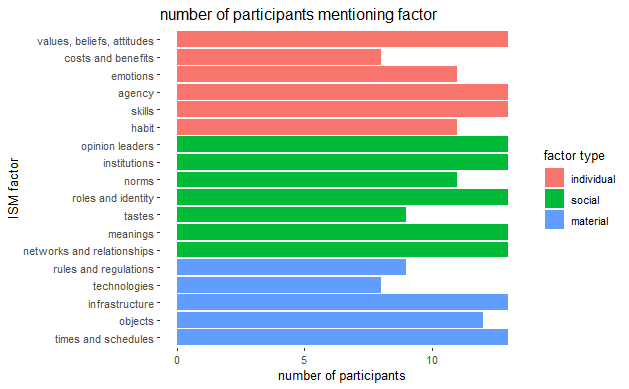
\includegraphics[width=1\linewidth]{figures/participants_mentioning_ism_factor.png}
    \caption{Number of participants mentioning ISM factors}
    \label{fig:ismparticipantcount}
\end{figure}

\begin{figure}[!ht]
    \centering
    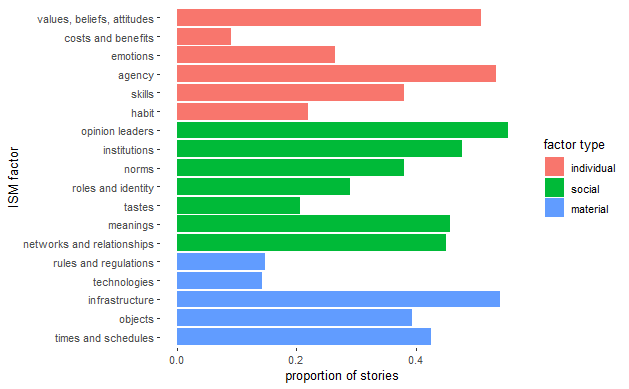
\includegraphics[width=1\linewidth]{figures/stories_mentioning_ism_factor.png}
    \caption{Number of stories mentioning ISM factors}
    \label{fig:ismstorycount}
\end{figure}

\begin{figure}[!ht]
    \centering
    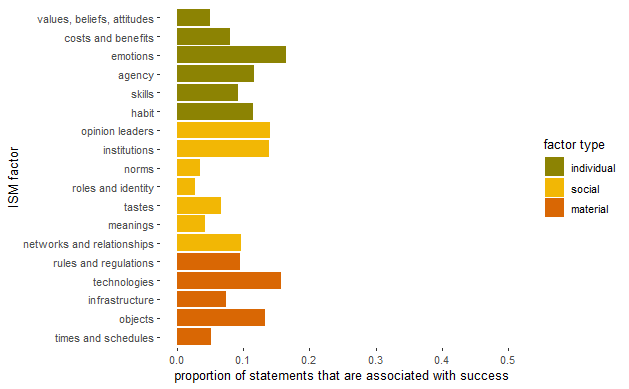
\includegraphics[width=1\linewidth]{figures/statements_associated_with_success.png}
    \caption{Proportion of statements for each ISM factor that are associated with success}
    \label{fig:ismsuccess}
\end{figure}

\begin{figure}[!ht]
    \centering
    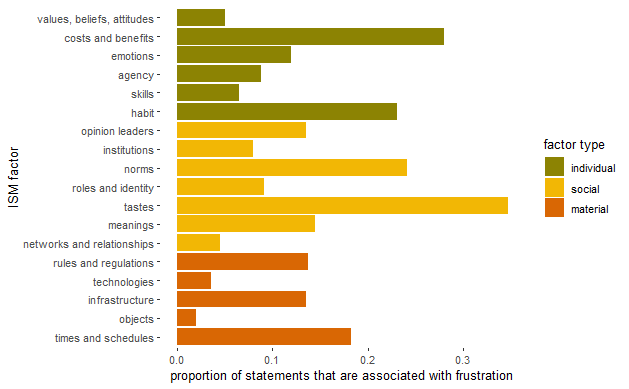
\includegraphics[width=1\linewidth]{figures/statements_associated_with_frustration.png}
    \caption{Proportion of statements for each ISM factor that are associated with frustration}
    \label{fig:ismfrustration}
\end{figure}

\begin{figure}[!ht]
    \centering
    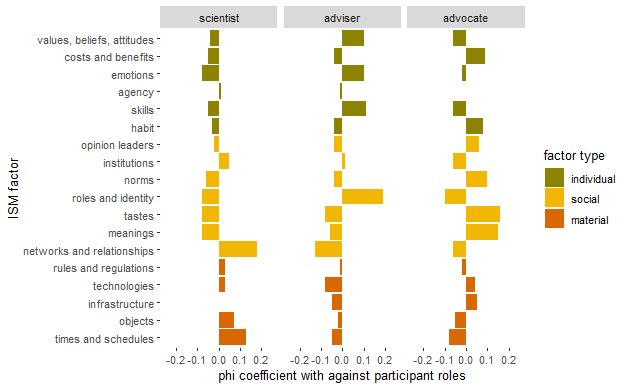
\includegraphics[width=1\linewidth]{figures/phi_coefficient_with_roles.png}
    \caption{Phi coefficient of participants' roles with ISM factors}
    \label{fig:ismparticipantcount}
\end{figure}

%\begin{figure}[!ht]
%    \centering
%    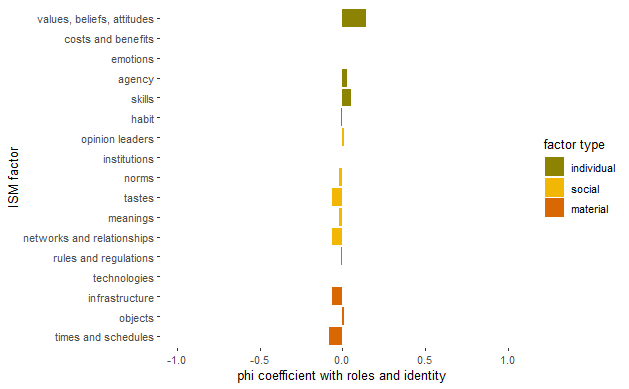
\includegraphics[width=1\linewidth]{figures/phi_coefficient_with_rolesandidentity.png}
%    \caption{Phi coefficient for each ISM factor against \ismsr}
%    \label{fig:ismphiroles}
%\end{figure}

%\begin{figure}[!ht]
%    \centering
%    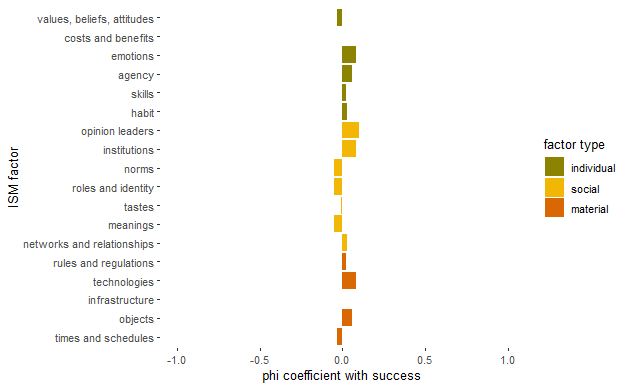
\includegraphics[width=1\linewidth]{figures/phi_coefficient_with_success.png}
%    \caption{Phi coefficient for each ISM factor against success}
%    \label{fig:ismphisuccess}
%\end{figure}

%\begin{figure}[!ht]
%    \centering
%    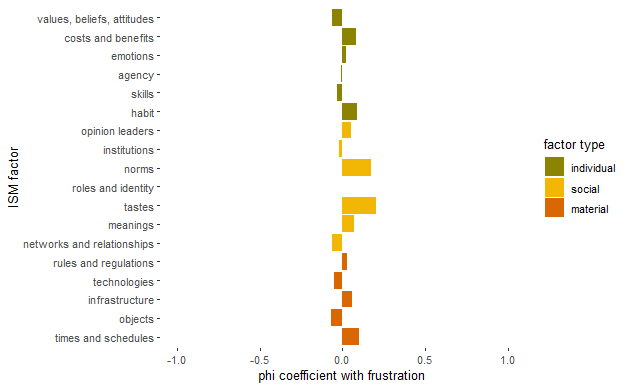
\includegraphics[width=1\linewidth]{figures/phi_coefficient_with_frustration.png}
%    \caption{Phi coefficient for each ISM factor against frustration}
%    \label{fig:ismphifrustration}
%\end{figure}

The ISM framework\improvement{make sure this is explained and referenced in Chapter~\ref{ch:lit} and how I used it is described in Chapter~\ref{ch:methods}} was used to identify the behaviour factors that enable or inhibit engagement and influence at the science policy interface. Figure~\ref{fig:ismstorycount} shows the number of stories in which each factor was mentioned. Each section below describes the nature of the drivers for each of 18 behavioural factors, as identified in the interviews.

Each the ISM factor was mentioned by at least half the participants.

\subsection{Individual factors}\label{sec:resindividual}

A wide range of factors relating to the individual participants' motivation were identified in the interviews. All participants identified \ismiv, \ismia{} and \ismis.  \ismiv{} and \ismia{} appeared in more than half the stories. \ismic{} was the least mentioned of all the ISM factors. Both \ismis{} and \ismih{} included observations the influences that the \ismis{} and \ismih{} of others had the quality of engagement.

\subsubsection{\ismiv}\label{sec:resismvalues}

\begin{table}[!ht]
\footnotesize
\caption{The main examples of \ismiv{} that influences CAN science and policy  engagements found in the interviews and example quotes}\label{tab:resvalues}
\begin{tabular}{L{.06\linewidth}L{.3\linewidth}L{.12\linewidth}L{.52\linewidth}} \hline
\textbf{id} & \textbf{\ismiv} & \textbf{influence} & \textbf{example quote} \\ \hline \hline 
iv1 & duty to try & enabling & \tquote{it's better to try than not try}{p03}{143} \\[5mm]
iv2 & moral imperative & enabling & \tquote{it would be morally not possible to not want to do the engagement if you knew the things I found out}{p08}{131} \\[5mm]
iv3 & social justice & enabling & \tquote{with very strongly held contested views on both sides of the debate ... it's actually rewarding in that often you can help to find a common ground}{p13}{68} \\[5mm]
iv4 & science should be useful (in general) & enabling & \tquote{when we're writing papers now, we want to make sure that they're going to be useful to to policy makers}{p02}{64} \\[5mm]
iv5 & science should be relevant & various & \tquote{in that programme we were thinking about the science but we tailored the questions that we asked so that they would have policy relevance}{p13}{15} \\[5mm]
%iv8 &  & inhibiting & \tquote{I look around madly, how can I get technology into my research so I can get it funded? I need technology ... because if I don't, I don't have any relevance}{p11}{70} \\[5mm]
iv6 & science should be credible & neutral & \tquote{I very much had to ground myself in what the science was saying and not say the UK government isn't doing enough}{p04}{29} \\[5mm]
iv7 & science should be open & neutral & \tquote{I've always really felt it important to make sure that the science that we do, that people know about it, that it doesn't just end up in an academic paper}{p14}{5} \\[5mm]
iv8 & science should be responsible & neutral & \tquote{you need to do the work and do as you start doing it, think about the environmental and societal impacts of it}{p01}{109} \\[5mm]
iv9 & we should challenge current policy approaches & neutral & \tquote{everyone would have some doubts about the strength of the pure cost benefit analysis approach to a climate problem}{p08}{95} \\[5mm]
iv10 & it is important to share what I know & enabling & \tquote{I have a few key messages and I want to try to do something with them}{p05}{102} \\[5mm]
iv11 & policy should be based on the best science & enabling & \tquote{one of the best ways that you can actually have long term impact on policy is by doing the the fundamental science that is going to be needed to inform long term policy decisions}{p13}{18} \\[5mm]
iv12 & we should be pragmatic & various & \tquote{lobbying sounds like a dirty word, but we're lobbying based on the best available science}{p06}{92} \\[5mm]
iv13 & value for public money & neutral & \tquote{this is mostly taxpayers money, it should be useful}{p07}{48} \\[5mm] \hline
\end{tabular}
\end{table}


Participants stated a range of \ismiv{} that motivated them to undertake policy-relevant science and engage with policy, such as a values relating to duty (iv1), moral imperative (iv2), and social justice (iv3). Many participants expressed beliefs about their science, such as that it should be useful (iv4), relevant (iv5), credible (iv6), open (iv7) and responsible (iv8). Engagements with policy were often driven by a belief that it is important to share knowledge (iv10) and that policy should be based on the best science (iv11). Finally, participants also acknowledge some attitudes to their work about being pragmatic (iv12) and returning value for public money.

\paragraph{Strategies:}
Because, in most cases, \ismiv{} had an enabling or neutral influence on engagements, strategies related to them tended to be to align to those values, beliefs or attitudes, and these therefore have not been further tabulated in this section. For instance, \tref{a participant who felt strongly that science should be credible}{p09} used a strategy \tquote{not to mislead, willingly or unwillingly}{p09}{74}.

\subsubsection{\ismic}\label{sec:resismcab}

\begin{table}[!ht]
\footnotesize
\caption{The main examples of expressions of \ismic{} that influences CAN science and policy engagements found in the interviews and example quotes}\label{tab:rescosts}
\begin{tabular}{L{.06\linewidth}L{.3\linewidth}L{.12\linewidth}L{.52\linewidth}} \hline
\textbf{id} & \textbf{\ismic} & \textbf{influence} & \textbf{example quote} \\ \hline \hline 
icb1 & too much effort & inhibiting & \tquote{life's too short and there's too much hard work to do on the research, to spend too much of your time [strategically targeting policymakers]}{p08}{50} \\[5mm]
icb2 & is the effort worth it? & various & \tquote{governments have enough information on which to act already and have quite sufficient evidence}{p04}{48} \\[5mm]
icb3 & its worth it & enabling & \tquote{If it's going to be useful, why wouldn't we prioritise our time to do that paper rather than something else}{p01}{78} \\[5mm] \hline
\end{tabular}
\end{table}

A weighing up of \ismic{} didn't feature a great deal in the interviews. Where it did, it tended to be about the effort it takes to engage with policy, against the worth of the outcomes. These range from feeling some aspects of engagement were too much effort (icb1), or worth the effort (icb3), or questioning whether the effort is worthwhile (icb2). Most participants stating only one position, \tref{although one participant stated all three positions}{p08}. 

\begin{table}[!ht]
\footnotesize
\caption{The strategies related to \ismic{} found in the interviews and example quotes}\label{tab:rescostsstrat}
\begin{tabular}{L{.06\linewidth}L{.3\linewidth}L{.64\linewidth}} \hline
\textbf{id} & \textbf{strategy} & \textbf{example quote} \\ \hline \hline
icbs1 & spreading the opportunities for success & \tquote{policy can be super powerful and continue perhaps to put the prime emphasis on those actors, but wouldn't put all my eggs in that basket}{p08}{144} \\[5mm] \hline
 \end{tabular}
\end{table}

\paragraph{Strategies:}
Two participants had strategies that spread opportunities for success (icbs1), which tended to involve engaging with a range of actors, not just those directly making policy decisions.

%There was very little indication of scientists weighing up the costs and benefits of their work or that of others. One scientist balanced the value of their activity with its used for policymaking and concluded that \emph{it's worth it} - \tquote{If it's going to be useful, why wouldn't we prioritise our time to do that paper rather than something else}{p01}{}, this was linked to an acknowledgement of the costs and benefits to policymakers for whom reading all the relevant scientific literature is \emph{too much effort}. Regarding engaging at the science policy interface, another scientist felt that they were \emph{not sure its worth the effort} - \tquote{I'm not convinced that it overall is hugely impactful}{p03}{}

\subsubsection{\ismie}\label{sec:resismemotions}

\begin{table}[!ht]
\footnotesize
\caption{The main examples of \ismie{} that influences CAN science and policy  engagements found in the interviews and example quotes}\label{tab:res****}
\begin{tabular}{L{.06\linewidth}L{.3\linewidth}L{.12\linewidth}L{.52\linewidth}} \hline
\textbf{id} & \textbf{\ismie} & \textbf{influence} & \textbf{example quote} \\ \hline \hline 
ie1 & curiosity; gratitude; pride; satisfaction; determination & enabling & \tquote{it is ultimately rewarding to get involved in some of the really knotty challenges where there's a lot of controversy}{p13}{67} \vfill \tquote{I'm proud of it because it was a beautiful thing that we created and a process that was really interesting
}{p05}{108} \\[5mm] 
ie2 & surprise; disappointment; despair; frustration; exhaustion & inhibiting & \tquote{I'm just kind of disappointed that with policy … in the UK, we get there but its very, very complex}{p08}{72} \vfill \tquote{I look around me and I see the promises of 20-30 years just gone}{p11}{84} \\[5mm] \hline
\end{tabular}
\end{table}

Various \ismie{} were associated with undertaking science and engaging with policy, often as a response to the experiences. Some of these were positive experiences and often provided motivation to continue with engagements (ie1). Other were experienced as demotivators and inhibitors (ie2).

\paragraph{Strategies:}
Because \ismie{} tended to be experience in response to experiences related to policy engagements, there were no strategies given to directly address the experience of emotions. However, strategic actions (related to other ISM factors) could result in experiences of pride and satisfaction.

\subsubsection{\ismia}\label{sec:resismagency}

\begin{table}[!ht]
\footnotesize
\caption{The main examples of \ismia{} that influences CAN science and policy  engagements found in the interviews and example quotes}\label{tab:resagency}
\begin{tabular}{L{.06\linewidth}L{.3\linewidth}L{.12\linewidth}L{.52\linewidth}} \hline
\textbf{id} & \textbf{\ismia} & \textbf{influence} & \textbf{example quote} \\ \hline \hline 
ia1 & having capability & enabling & \tquote{we're certainly getting them thinking}{p08}{90} \\[5mm]
ia2 & happenstance & various & \tquote{really so much of the policy process is about being in the right place at the right time}{p10}{55} \\[5mm]
ia3 & limits to my influence & inhibiting & \tquote{I don't know whether I can really claim that my specific research has impacted}{p12}{39} \\[5mm] \hline
\end{tabular}
\end{table}

\ismia{} was the most commonly expressed individual influence in terms of stories. This influence could be enabling, with participants expressing how they have confidence in their ability (ia1), inhibiting, where participants identified that their influence is limited (ia3), or they identified the influence of chance on a number of aspects of their work, particularly the ability to engage with policy (ia2).

\begin{table}[!ht]
\footnotesize
\caption{The strategies related to \ismia{} found in the interviews and example quotes}\label{tab:resagencystrat}
\begin{tabular}{L{.06\linewidth}L{.3\linewidth}L{.64\linewidth}} \hline
\textbf{id} & \textbf{strategy} & \textbf{example quote} \\ \hline \hline
ias1 & making it happen & \tquote{making sure that when policy windows or relationships emerge, that you can leverage them or you can use them to influence policy}{p12}{83} \\[5mm] \hline
 \end{tabular}
\end{table}

\paragraph{Strategies:}
Given the influence of chance the initiation and outcomes of engagements with policy, a number of participants identified that they tried to be ready for openings for engagement (ias1), which relates to building knowledge in the policymaking process (Section~\ref{sec:resismskills}) and anticipating changes in policy (Section~\ref{sec:resrules}).

\subsubsection{\ismis}\label{sec:resismskills}

\begin{table}[!ht]
\footnotesize
\caption{The main examples of observations related to \ismis{} that influences CAN science and policy  engagements found in the interviews and example quotes}\label{tab:res****}
\begin{tabular}{L{.06\linewidth}L{.3\linewidth}L{.12\linewidth}L{.52\linewidth}} \hline
\textbf{id} & \textbf{observation} & \textbf{influence} & \textbf{example quote} \\ \hline \hline 
is1 & I know and understand the science & enabling & \tquote{actually we're probably the best people to be speaking to}{p01}{43} \\[5mm]
is2 & I know and understand the policymaking process & enabling & \tquote{because we've been speaking to some of the policy people as part of that, we knew this is just setting the policy landscape}{p01}{86} \\[5mm]
%is3 & the policymaker knows and understands the area of policy & enabling & \tquote{what are we going to do when [policy official] goes, he's the glue. All of these fresh, young things that constantly appear and move on and move on, there's very few of those stable kind of people with that legacy knowledge of what we did last time or how things were before}{p14}{108} \\[5mm]
is3 & the policymaker can gain knowledge easily & enabling & \tquote{there is a receptivity to that argument, particularly amongst the bright people in the civil service - they totally get that}{p08}{107} \\[5mm]
is4 & I need to gain knowledge in the science & neutral & \tquote{I do need to be in touch with colleagues and coming into the office and stay in contact with them and ask some questions about things to try and draw out what it is that might be of interest}{p07}{35} \\[5mm]
is5 & I need to gain knowledge in the policymaking process & inhibiting & \tquote{it felt like we were worlds apart in terms of what we could provide and what they really needed and also the language that they speak was very different to ours}{p04}{61} \\[5mm]
is6 & the policymaker needs to gain knowledge in the science & inhibiting & \tquote{I realised there's a huge challenge there in terms of just understanding each other's domain, so that we understand what they need and we and likewise they can understand the limits of what we can provide}{p04}{61} \\[5mm]
 \hline
\end{tabular}
\end{table}

\ismis{} was interpreted as being largely about knowledge, both of CAN science and of policymaking processes. These were influential because lack of the right knowledge made engagement considerably harder. In particular, participants understand the relevant science (is1) or policymaking process (is2) was, understandably, beneficial to engagement, as was working with policy people who cold gain new knowledge easily (is3). Where participants expressed that they need to gain scientific knowledge (is5), this wasn't seen has inhibiting, simply part of their role. However, barriers to engagement were noted when the participant felt they needed to understand the policymaking process better (is5) or when working with policymakers who needed to gain more knowledge about relevant science (is6). 

\begin{table}[!ht]
\footnotesize
\caption{The strategies related to \ismis{} found in the interviews and example quotes}\label{tab:resskillsstrat}
\begin{tabular}{L{.06\linewidth}L{.3\linewidth}L{.64\linewidth}} \hline
\textbf{id} & \textbf{strategy} & \textbf{example quote} \\ \hline \hline
iss1 & working together to build knowledge & \tquote{We scoped out the research with them - they had a quite a clear idea about what they wanted to achieve}{p05}{27} \\[5mm] \hline
 \end{tabular}
\end{table}

\paragraph{Strategies:}
Apart from the very direct strategy of gaining those missing skills, some participants described how they worked together with policymakers to develop the knowledge needed. This is closely related to the strategy of coproduction (Section~\ref{sec:restechnologies}).

\subsubsection{\ismih}\label{sec:resismhabit}

\begin{table}[!ht]
\footnotesize
\caption{The main examples of \ismih{} that influences CAN science and policy  engagements found in the interviews and example quotes}\label{tab:reshabit}
\begin{tabular}{L{.06\linewidth}L{.3\linewidth}L{.12\linewidth}L{.52\linewidth}} \hline
\textbf{id} & \textbf{\ismih} & \textbf{influence} & \textbf{example quote} \\ \hline \hline 
ih1 & scientists doing science for scientists & various & \tquote{you're doing science and you're publishing papers and the people who read those papers are only doing it because they need stuff to cite their study}{p03}{122} \\[5mm]
ih2 & scientists applying the deficit model to create change & various & \tquote{you'd think: give the policymaker the information and they'll act}{p05}{95} \\[5mm]
ih3 & policy obtaining information from the same sources & various & \tquote{I was like, where's the social science in here, you keep bringing in the physical academies and not the social science}{p06}{60} \\[5mm]
ih4 & policymakers using the same policymaking approach & various & \tquote{…they'll just continue to do the same thing and make the same mistakes or have the same assumptions about what works to change behaviour}{p05}{85} \\[5mm]
 \hline
\end{tabular}
\end{table}

\ismih{} was interpreted as behaviours that were particular to either scientists or policymakers that could often go unquestioned - except that they were identified by participants precisely because they were questioning them.  Four main \ismih{} types were identified within the interviews, two being habits of scientists and two of policymakers. Firstly, there can be a tendency for science to be produced only for scientists (ih1). It was also noticed that scientists could habitually use a model of policy change based solely on the idea that not enough information is available to policymakers (ih2). Policymakers were observed going to the same sources for their information and evidence (ih3) as well as using the same approaches (1h4) such as particular economic models.

\begin{table}[!ht]
\footnotesize
\caption{The strategies related to \ismih{} found in the interviews and example quotes}\label{tab:reshabitstrat}
\begin{tabular}{L{.06\linewidth}L{.3\linewidth}L{.64\linewidth}} \hline
\textbf{id} & \textbf{strategy} & \textbf{example quote} \\ \hline \hline
ihs1 & open to new ideas & \tquote{[you're] looking for other ways of tackling things, taking a different perspective on things}{p07}{7} \\[5mm]
\hline
 \end{tabular}
\end{table}

\paragraph{Strategies:}
To break out of habits, participants noted their own, and others', efforts to find new ideas and ways of working (ihs1).
 
\subsection{Social factors}\label{sec:ressocial}

Many factors relating to participants social links were identified in the interviews. All participants identified \ismso, \ismsi, \ismsr, \ismsm{} and \ismsnr{}. ,  

\subsubsection{\ismso}\label{sec:resopinionleaders}

\begin{table}[!ht]
\footnotesize
\caption{The 7 types of mention of \ismso{} in the interviews and example quotes for each type}\label{tab:resopinionleaders}
%\begin{tabularx}{\textwidth} {DIQ} 
\begin{tabular}{L{.06\linewidth}L{.3\linewidth}L{.12\linewidth}L{.52\linewidth}} \hline 
\textbf{id} & \textbf{observation} & \textbf{influence} & \textbf{example quote} \\ \hline \hline 
ol1 & scientists' knowledge   drew interest from policymakers & enabler & \tquote{They had already decided they wanted to work with us}{p05}{26}  \\[5mm]
ol2 & scientists influencing policymakers & enabler & \tquote{Informally I think they [have been] picked up and had a bit of traction}{p03}{37}  \\[5mm]
ol3 & scientists influencing others & enabler & \tquote{We've been cited by both industry and NGOs on different sides of the debate, so we've probably got something right there}{p01}{70} \\[5mm]
ol4 & senior scientists are more likely to be   listened to & enabler & \tquote{When it comes to something for more formal like that, they tend to go for the professors}{p03}{75} \\[5mm]
ol5 & I look up to other scientists & enabler & \tquote{He's an excellent scientist, he's very inclusive and he's   incredibly motivational from a scientific perspective, very much in favour of community building}{p04}{54} \\[5mm]
ol6 & others influence policymakers & inhibitor & \tquote{Sometimes what they bring is politically convenient, and policymaking is not just about evidence is also about political convenience   or political opportunity. They provide narratives to use or discard certain evidence}{p09}{113} \\[5mm]
ol7 & policymakers have influence & neutral & \tquote{I think policy makers have the greatest leverage of all}{p08}{135} \\[5mm] \hline
\end{tabular}
\end{table}

\begin{table}[!ht]
\footnotesize
\caption{The strategies related to \ismso{} found in the interviews and example quotes}\label{tab:resopinionstrat}
\begin{tabular}{L{.06\linewidth}L{.3\linewidth}L{.64\linewidth}} \hline
\textbf{id} & \textbf{strategy} & \textbf{example quote} \\ \hline \hline
ols1 & opportunities to promote my/our work & \tquote{If I get media requests, I think if I've got the expertise, I should do that because it goes with the job}{p01}{41}  \\[5mm]
ols2 &  opportunities to understand the perspectives of policymakers & \tquote{we try and find out what their priorities are}{p12}{11} \\[5mm] \hline
\end{tabular}
%\end{tabularx}
\end{table}
\improvement{the layout of this table needs to be easier to read}

Nearly half of the stories mention individuals and groups to whom scientists and policymakers will reach out, and be influenced by - more than any other social factor. This indicates that opinion leaders are important to scientists engaging with policy. Given the criteria for inviting people to take part in this study, it is not surprising that many participants mentioned being invited by policymakers to share their knowledge (ol1). Others identified that they believed they had had some influence on policymaking (ol2) or others, such as industry and NGOs (ol3). The was specific recognition that senior scientists are more likely to have influence (ol4).  

It was also quite common to observe that there are non-science actors, such as other governments, industry, learned societies, research councils, special advisers and NGOs, who have influence in the decisions being make (ol6). Further, policymakers themselves were considered to have influence (ol7)

\paragraph{Strategies:}
In some cases, this understanding has been used to gain influence. A number of participants mentioned promoting their work through third parties such as media opportunities but also by engaging with organisations such as industry or NGOs such as charities, campaigning organisations and networks (think tanks) as a mechanism for influencing policymaking (ols1). A different approach was to make efforts to align with policymakers by taking up opportunities to listen to their perspectives (ols2).

\subsubsection{\ismsi}\label{sec:resinstitutions}

\begin{table}[!ht]
\footnotesize
\caption{The main influences that \ismsi{} represented in the interviews and example quotes for each type}\label{tab:resinstitutions}
\begin{tabular}{L{.06\linewidth}L{.3\linewidth}L{.12\linewidth}L{.52\linewidth}} \hline
\textbf{id} & \textbf{observation} & \textbf{influence} & \textbf{example quote} \\ \hline \hline 
i1 & within my institution there is an expectation (to engage with policy; to maintain neutrality; to avoid some topics; to create impact; to write papers; to represent it at events; to write briefings) & various & \tquote{that was very much the culture of that centre was doing work [that] was trying also to impact the world outside academia}{p10}{14} \\[5mm]
i2 & evaluation of our work (by demonstrating impact; by citations; by identifying where we have been influential; by process not outcome; by outputs; by publications) & enabling & \tquote{I've picked up on, certainly from the Research Council … I think all of probably UKRI, policy engagement seems to have the same sort of value as industry engagement}{p01}{103} \\[5mm]
i3 & evaluation of our work (by CAN outcomes; can be ambiguous) & inhibiting & \tquote{having meetings with government departments or sitting on advisory committees, you can't always say `see this piece of advice that has led to this action'}{p05}{23} \\[5mm]
i4 & the evaluation of policy (is very limited; is limited to the obligation to respond; is focused on measureable policy outcomes) & inhibiting & \tquote{they often just don't even evaluate their policies}{p05}{83} \hfill \tquote{the policy makers need measurable things - organisations, to be accountable, need data and statistics}{p11}{33} \\[5mm]
i5 & the evaluation of policy (was possible by giving feedback) & enabling & \tquote{They took every recommendation we had. That was really impactful, albeit in a very tiny area}{p05}{68} \\[5mm]
i6 & policy institutions (have distinct ways of working; are changing slowly; are functioning on limited resources) & various & \tquote{I found the ... hierarchy quite interesting - in a meeting, why is someone else saying what I could just say, why do I have to write the notes so that they can say it ... you have to prepare all these briefings and notes for people to say}{p06}{58} \\[5mm]
i7 & the policy process (has defined timeframes; has defined subject frames; has defined roles) & various & \tquote{you can write the the nicest paper and write the nicest briefing and the nicest translation of that, but people won't listen to you because the decision has been made}{p09}{93} \\[5mm]
i8 & the policy process (is difficult to understand) & inhibiting & \tquote{I think it's often very difficult to know how advice gets used}{p05}{22} \\[5mm]
i9 & we are able to choose our field of research & enabling & \\[5mm]
i10 & we have a social responsibility as a public organisation & neutral & \\[5mm] \hline
\end{tabular}
\end{table}

\begin{table}[!ht]
\footnotesize
\caption{The strategies \ismsi{} with example quotes for each}\label{tab:resinstitutionstrat}
\begin{tabular}{L{.06\linewidth}L{.3\linewidth}L{.64\linewidth}} \hline
\textbf{id} & \textbf{strategy} & \textbf{example quote} \\ \hline  \hline
is1 & engage with policy where possible & \tquote{maybe we'll ask them to sit on an Advisory Board}{p12}{7} \\[5mm]
is2 & select policy-related research topics & \tquote{we'd focus on the areas to do with [the biophysical environment], choosing things where we knew that humans might want to interact}{p13}{17} \\[5mm]
is3 & produce evidence that is relevant and timely & \tquote{be aware of the window of opportunity you have to provide evidence that can contribute to the conversation. At some point certain conversation is concluded}{p09}{92} \\[5mm]
is4 & focus on creating a good process (and less so on outcome) & \tquote{that's success for me basically catalysing a constructive, evidence-based sincere discussion of the options}{p09}{50} \\[5mm]
\hline
\end{tabular}
\end{table}

Institutions had a range of influences on participants. Their own institutions exerted a range of expectations (i1), the most common, unsurprisingly, was an expectation to engage with policy. Other expectations related to the institution type. Those participants in academic institutions were expected to create and demonstrate impact and write papers. Those participants in government-related institutions were expected to maintain neutrality when speaking or writing about their work. \tref{One participant}{p11} commented how there was an unspoken pressure on scientists to stick to certain topics of research and publication, and avoid others. There was also desire to find ways to evaluate engagements at the policy interface, arising from a various institutional contexts (not least that policy itself often expects evaluation) (i2). Many of these were related to REF and UKRI requirements (unsurprisingly, since several participants were selected on the basis of REF and UKRI case studies). Participants also referred to being cited or being able to identify (or suspecting) their influence in particular policy statements. However, several participants stated that they found it very difficult to evaluate their impact because of ambiguities in the science to policy [journey] and two participants also noted that the ultimate impact, that CAN issues were lessening, was not being made (i3). Participants noted that they didn't witness much evaluation of policy (i4) except in one case (with Scottish Government) when their recommendations were accepted (i5).

The influence of policy institutions on engagement were mentioned by several participants, most often identifying a range of novel ways of working (which were often much more formal and structured than participants' own institutions) (i6). These were reflected in the references to the policy process which was perceived as either highly structured (i7) having defined subject and time frames, and roles, or as being difficult to understand (i8).

Other institutional influences included researchers having the ability to define their own research field (i9), the recognition of the social responsibilities of public organisations (i10) and public funding, and contractual obligations.

\paragraph{Strategies:} Often, the mentioned influences of institutions appeared to have strategic origins. For instance, the expectation to engage with policy, maintain neutrality, produce documents, and evaluate engagements could all be expected to support positive outcomes of policy engagement (is1). In a number of cases participants had mentioned their ability to choose their field of research because they had used this ability to select policy-relevant lines of enquiry (is2). Several participants advised on providing evidence to policy that met needs in terms of topic and timing (is3). \tref{In reponse to the difficulty with identifying successful outcomes, one participant described how they focussed on creating a well-informed discussion within the policy process}{p09}.

\subsubsection{\ismsn}\label{sec:resnorms}

\begin{table}[!ht]
\footnotesize
\caption{The main examples of \ismsn{} that influences CAN science and policy engagements found in the interviews and example quotes}\label{tab:resnorms}
\begin{tabular}{L{.06\linewidth}L{.3\linewidth}L{.12\linewidth}L{.52\linewidth}} \hline
\textbf{id} & \textbf{observation} & \textbf{influence} & \textbf{example quote} \\ \hline \hline 
sn1 & what politicians would accept in terms of policy and policy instruments & inhibitor & \tquote{we cannot regulate in this area, we cannot actually stop people from doing things, that would just be impossible to say to a minister}{p05}{73} \\[5mm]
sn2 & what the electorate would accept, or at least politicians' perceptions of what the electorate would accept & inhibitor & \tquote{if the farmers don't want to plant it because it's culturally not right for them or the people don't like the look of it in the countryside and they don't want it, or the policy makers don't believe it because there's all the Panorama and all the negative [media] - biomass is really hot potato politically}{p14}{34} \\[5mm]
sn3 & doing research is more valued than advising policymakers & neutral & \tquote{climate modelling: Proper science; Working with behaviour: only proper science if you do it quantitatively through anonymous surveys where you can do p-stats, anovas; Talking to communities: [not proper science]...}{p11}{68} \\[5mm]
 \hline
\end{tabular}
\end{table}

The majority of \ismsn{} expressed were perceptions of what politicians would accept in terms of policy and policy instruments (sn1). These were often linked to perceptions of what the electorate would accept, or at least politicians' perceptions of what the electorate would accept (sn2). These norms were closely related, and difficult to untangle from the tastes of policymakers as perceived by participants (Section~\ref{sec:restastes}). There were also hints at norms for scientists. These related to scientists roles such as doing research is more valued than advising policymakers, as well as what is considered \tquote{proper science}{p11}{68} (sn3). No specific strategies were identified relating to \ismsn.

\subsubsection{\ismsr}\label{sec:resroles}

\begin{table}[!ht]
\footnotesize
\caption{The main examples of \ismsr{} that influences CAN science and policy  engagements found in the interviews and example quotes}\label{tab:res****}
\begin{tabular}{L{.12\linewidth}L{.3\linewidth}L{.58\linewidth}} \hline

\textbf{id} & \textbf{\ismsr} & \textbf{example quote} \\ \hline \hline
roles & academic; adviser; advocate; citizen; public servant; representative; researcher; specialist &  \\[5mm]
identities & authoritative; candid; esteemed; experienced; expert; helpful; humble; impartial; informed; judicious; receptive; relevant; selfish & \\[5mm] \hline
\end{tabular}
\end{table}


Participants referred to theirs, or other scientists', roles or identity in about one fifth of the stories. The nature of the roles were varied. As one participant noted \tquote{scientists are a very diverse bunch}{p09}{60}. Participants saw their roles, and those of other scientists, as a \emph{researcher}, who is sometimes a \emph{specialist}. Some roles are in relation to the scientists' institution, such as \emph{academic}, \emph{representative} and \emph{public servant}, the latter referring to a scientist in a government science setting or in an academic institution with a strong awareness of its public funding (See also Section~\ref{sec:resismvalues} \emph{value for public money} and Section~\ref{sec:resinstitutions} \emph{social responsibility of public organisations}). Those working more regularly at the interface with policy, may consider themselves more as an \emph{adviser} and occasionally an \emph{advocate}. Also, a number of participants were conscious of their role as a \emph{citizen}.

Scientists' identities ranged from those largely within the scientific realm concerning scientific recognition (\emph{esteemed}), ability (\emph{expert}) and duty (\emph{helpful}), to those that emerged at the interface concerning the ability to gain notice (\emph{authoritative}), be trusted (\emph{capable}, \emph{credible}), know the processes of policy (\emph{experienced}, \emph{informed}), align with the perspectives of policy (\emph{receptive}, \emph{relevant}) and balance professional demands (\emph{impartial}, \emph{judicious}). This latter pair of identities somewhat contrasted with an observation that some scientists are, or have the opportunity to be, \emph{candid} about their views of CAN science-policy. Finally, being \emph{humble} and \emph{selfish} were identified as contrasting identities of scientists don't or do who promote themselves. The identities \emph{expert}, \emph{authoritative} and \emph{candid} were more commonly applied to other scientists when providing examples of identities of scientists at the science-policy interface. All identities, except an instance of \emph{candid}, and the instances \emph{humble} and \emph{selfish}, were referred to positively.

\begin{table}[!ht]
\footnotesize
\caption{The strategies related to \ismsr{} found in the interviews and example quotes}\label{tab:resrolesstrat}
\begin{tabular}{L{.06\linewidth}L{.3\linewidth}L{.64\linewidth}} \hline
\textbf{id} & \textbf{strategy} & \textbf{example quote} \\ \hline \hline
srs1 & do deeper, more policy-focused, research & \tquote{but a lot of scientists should actually get on and try and discover what they think is going to be societally important stuff and it'll have policy influence through that}{p13}{} \\[5mm]
srs2 & identifying preferred role and sticking to it & \tquote{But beyond that, I consciously draw the line [between advice and advocacy]}{p09}{} \\[5mm]
srs3 & identifying the bounds of advocacy & \tquote{[I advocate] only within already societally-established parameters}{p09}{} \\[5mm]
srs4 & making a conscious pivot in role & \tquote{I have pivoted, but that's just because the demand isn't ... from ... policy makers asking me questions or trying to set a policy agenda}{p08}{} \\[5mm]
srs5 & collaborating with people in other roles & \tquote{It's a bit toe curling, which is why we also work with a charity ... who do a lot more of that}{p05}{}\\[5mm] \hline
\end{tabular}
%\end{tabularx}
\end{table}

\paragraph{Strategies:}
The strategies suggested in relation to role conflicts, were to address concerns that scientists who \emph{advocate} are less credible or that they devalue science or evidence that they convey. The first of these was to focus on fundamental research that would ultimately have policy-relevance (srs1). The related advice given was that research can lead to self-evident policy decisions whilst being entirely neutral. The second strategy was to be very clear about which role the scientist prefers and identify the boundaries to that role (srs2). This would be to choose to be either an advisor or an advocate. Another strategy is to advocate but within strict boundaries (srs3). For instance, this may be advocating for specific principles or area of knowledge to be included as evidence, a particular issue to be put on the agenda or a new approach to policymaking. Several participants had changed role, stepping away from scientific research, in order to have greater influence (srs4). Finally, working with NGOs who have greater flexibility to advocate (or even campaign) was considered propitious by some participants (srs5), meaning that the scientists could continue research and advise without personal conflict.

\subsubsection{\ismst}\label{sec:restastes}

\begin{table}[!ht]
\footnotesize
\caption{The main \ismst{} expressed in the interviews and example quotes}\label{tab:restastes}
\begin{tabular}{L{.06\linewidth}L{.3\linewidth}L{.12\linewidth}L{.52\linewidth}} \hline
\textbf{id} & \textbf{observation} & \textbf{influence} & \textbf{example quote} \\ \hline \hline
st1 & favouring progressive over moderate policies & various & \tquote{he idea of it was to try to push a boundary, a bit of what could be done more and be more ambitious}{p03}{24} \\[5mm]
st2 & favouring policy that creates social change over technological developments & various & \tquote{right of centre politically, we know there is just less willingness to intervene to change behaviour - that's what we've been contending with recently}{p05}{75} \\[5mm]
st3 & favouring public engagement for behaviour change over traditional approaches & various & \tquote{people need to be part of decision making, their lives are going to change and they have to be engaged in that and whether that's heat pumps or dietary change or whatever else it might be}{p03}{105} \\[5mm]
 \hline
\end{tabular}
\end{table}

On the whole, statements indicating \ismst{} related to conscious choices of how CAN issues were conceptualised by scientists and policymakers (often politicians) and the consequent preferences for CAN solutions, economic approaches, and democratic instruments. These tended to be referred to when there was a dichotomy between the participant's preference, and that of policymakers and politicians, or an observation that such policy tastes are changing and were also often related to perceived norms, as described in Section~\ref{sec:resnorms}. Mentions of \ismst{} were often associated with frustrations because they could severly limit the ability for some participants to engage with policy.

The main \ismst{} found in the interviews related to choices of policy approaches in general, with some participants indicating that they would prefer policy choices that better matched the urgency of CAN issues, rather than the moderate policy choices that they witnessed (st1). A number of participants specifically identified frustrations with the lasts governments' preference for technological solutions to CAN issues, over aspects of behaviour change (st2). These were particularly inhibiting to social scientists who found it more difficult to engage. Relatedly, a number of participants had tried to share their insights into public participation for developing policy but were inhibited by the lack of willingness of policy makers to engage deeply (st3). Instead, participants found that they were constrained to engaging with policymakers who were applying more traditional approaches to change behaviour (e.g. \tquote{they'll say, `our research priorities are labelling' and we'll try not to roll our eyes and say `but labelling really doesn't work'}{p05}{42}).

\begin{table}[!ht]
\footnotesize
\caption{The strategies related to \ismst{} found in the interviews and example quotes}\label{tab:restastesstrat}
\begin{tabular}{L{.06\linewidth}L{.3\linewidth}L{.64\linewidth}} \hline
\textbf{id} & \textbf{strategy} & \textbf{example quote} \\ \hline \hline
sts1 & challenging the economic approaches of policymakers & \tquote{they've been grown up enough to allow some conversation about the limitations [of current economic thinking] and the different ways of looking at it}{p08}{39} \\[5mm]
sts2 & establishing diverse engagements & \tquote{I'm deploying a more diverse strategy because the politicians have made choices, to not get this, or act on this, repeatedly}{p08}{136} \\[5mm]
 \hline
 \end{tabular}
\end{table}

\paragraph{Strategies:}
Few participants identified any strategies for addressing conflicting \ismst{} between themselves and policymakers. Two strategies suggested were to challenge the approaches used by policymakers (sts1) and to engage well beyond policy (sts2).

\subsubsection{\ismsm}\label{sec:resmeanings}

\begin{table}[!ht]
\footnotesize
\caption{The 7 main \ismsm{} related to CAN science and policy found in the interviews and example quotes}\label{tab:resmeanings}
%\begin{tabularx}{\textwidth} {DIQ} 
\begin{tabular}{L{.06\linewidth}L{.3\linewidth}L{.12\linewidth}L{.52\linewidth}} \hline
\textbf{id} & \textbf{meaning} & \textbf{influence} & \textbf{example quote} \\ \hline \hline 
m1 & CAN issues are serious & enabler &	\tquote{there is a broad consensus in policy and politics, climate change is important, and we should do stuff about it and things are happening, but that's a very long won battle and and it's still just that pretty basic level}{p03}{127} \\[5mm]
m2 & CAN issues are not serious & inhibitor & \tquote{That's not really engaging with what we said, but that's all they have to do, just write a written response. It doesn't really matter if it was a good response or a shitty response}{p05}{107} \\[5mm]
m3 & CAN issues are simple & inhibitor & \tquote{the core economics is telling you `put a uniform carbon price on everything and everything will be fine'}{p08}{112} \\[5mm]
m4 & CAN solutions are complex & inhibitor & \tquote{Suggesting a great solution to reducing emissions that destroys biodiversity - if you just look at carbon molecules, it looks fantastic, but obviously it's not something that policymakers should be implementing if they have already said that they want to protect that biodiversity as well. There are many of those interactions}{p09}{76} \\[5mm] \hline
\multicolumn{4}{L{\linewidth}}{\textbf{sets of meanings}} \\ \hline
m5 & CAN science framed with a scientists' meaning & varied & \tquote{more often I think it was a more vague `trying to push things here and there and hope they stick'}{p03}{82} \\[5mm]
m6 & the meaning of scientist & varied & \tquote{fairly independent and hopefully balanced}{p01}{121}  \vfill \tquote{treated as na\"ive and a bit like children}{p11}{45} \\[5mm]
m7 & the meaning of success	& varied & \tquote{the perspective to not consider success in terms of outcomes for myself, but really in terms of process}{p09}{46} \\ \hline
\end{tabular}
\end{table}

\unsure{rude word}

\begin{table}[!ht]
\footnotesize
\caption{The conflicts in \ismsm found in the interviews and example quotes for each}\label{tab:resmeaningsconf}
%\begin{tabularx}{\textwidth} {DIQ} 
\begin{tabular}{L{.06\linewidth}L{.3\linewidth}L{.64\linewidth}} \hline
\textbf{id} & \textbf{conflict} & \textbf{example quote} \\ \hline \hline 
mc1 & experiences of contrasting meanings & \tquote{the dominant way of thinking is not like thinking, `oh, this is thing we're called nature, that's our life support system and actually, we can't buy anything in the marketplace that can do what it does for us so maybe we should disproportionately value it for that reason', which would seem very intuitive}{p08}{121} \\[5mm]
mc2 & scientific evidence is only part of policy sensemaking & \tquote{ministers will have to make decisions based on lots of different pieces of evidence - science evidence is one of them}{p13}{39} \\[5mm]
mc3 & consequences of specific framing & \tquote{we have lost the battle for ideas that frame how we do research and what is acceptable research to do}{p11}{66} \\[5mm] \hline
\end{tabular}
%\end{tabularx}
\end{table}


There was a strong sense across the interviews that \emph{meaning} is important when conveying CAN knowledge across the science-policy interface. Within policy science, this translates to issue- and problem-framing. A number of very specific meanings were identified within the wider context of CAN science and CAN policy and Table~\ref{tab:resmeanings} describes the main 7 of these, which were held by the participants or were perceived to be held by those they engaged with. Specifically, there was a contrast between the those understanding CAN issues are to be serious or urgent (m1), which made engagement easier, and the view by some that they are not very important (m2), which made engagement difficult (including a reference to using CAN to ignite culture wars). Another meaning that participants noted was the perspective of policymakers that tended to simplify CAN issues to, often, those aspects that can be measured (carbon, trees, temperature) or to being able better modelling (m3). This could inhibit discussion, particularly when nuances of the scientific evidence ran contrary to the simplified view. In this case, the meaning to scientists is quite the opposite, that CAN issues are not simple. This is reflected in participants' understanding of CAN solutions, that they are complex (m4). Again, the need to convey such a meaning across the interface with policy could be inhibiting to smooth engagement. 

These 4 meanings were specific examples of perspectives held by participants that are likely to be some of the strongest drivers for many scientists working at the CAN policy interface. They are particularly potent for CAN scientists which is possibly why some participants stated that they themselves, or others that they knew, had not used policy framing for their engagements with policy (m5). On the whole, this was not considered an enabler to engagement, despite plain speaking being considered an asset by \tref{one participant}{p03}. 

Participants also noted that they themselves were given \emph{meaning} (m6), which could have a positive influence, such as being seen as credible, or a negative influence, such as being seen as na\"ive. They also actively considered the finding meaning in their work, with more positive experiences being described by those who focused on creating a successful engagement process than those who focused on a successful engagement outcome (m7).

\paragraph{Conflicts:}
As already noted, there were direct contrasts between the general meanings associated with CAN issues and solutions (i.e. the issue being serious versus the issue being trivialised and the issue being simplified versus the solutions being complex). Another area of conflict resulted from such specific meaning of CAN solutions (mc1; which is also reflected in Section~\ref{sec:restastes}). These were particularly related to the contrast between CAN issues having meanings related to human survival versus to economic imperatives, and whether solutions should involve citizen engagement or should be purely technological. These contrasts tended to be between the scientists' perspectives and the perspectives of policymakers. This may have been related to the acknowledgement by several participants that scientific evidence is often not the preeminent evidence used for making sense of CAN issues and policy (mc2). Participants also noted conflicts that arose from the more specific meanings, or framings, of CAN science and CAN policy (mc3). For instance, \tref{one participant noted that, the need to give research and its products meaning for policy, constrained the breadth of science that it was possible to engage with}{p11}. 

%	CAN solutions are technologies	\tquote{Government loves its technology, they love to announce some whatever billion pound fund for CCS or whatever}{p03}{61}
%	CAN solutions are behaviour change	
%	experiences of different meanings (technology versus behaviour change)	\tquote{It's been really frustrating because they've just wanted to solve the whole net zero problem from a very strong technological sense}{p12}{50}  \vfill  \tquote{But it was very, very, very difficult to get government to acknowledge that [we're not going to do the things we need to do on climate change without the involvement of people]}{p03}{66}


\begin{table}[!ht]
\footnotesize
\caption{The strategies to create \ismsm found in the interviews and example quotes for each}\label{tab:resmeaningsstrat}
\begin{tabular}{L{.06\linewidth}L{.3\linewidth}L{.64\linewidth}} \hline
\textbf{id} & \textbf{strategy} & \textbf{example quote} \\ \hline \hline 
ms1 & good evidence is policy-relevant & \tquote{unless there's a need they have or you frame it in a way that is aligned with what their current anxieties are, then they probably are not going to pay attention at all}{p05}{123} \\[5mm]
ms2 & good evidence is unbiased &  \tquote{you're in a much stronger position to go in with the most complete piece of scientific evidence you can present it neutrally to science to ministers or senior officials and let them then reach their own conclusions}{p13}{39} \\[5mm]
ms3 & creating evidence from science & \tquote{you … do the assessment of the knowledge and you take that science and you do the intellectual exercise of how much we believe, what alternatives are there available to look at this problem, how they differ in their answers, or maybe the answers are the same}{p09}{70} \\[5mm]
ms4 & creating meaning from science or evidence & \tquote{translate the evidence that we're giving into palatable messages}{p05}{74} \\[5mm]
ms5 & adjusting to context & \tquote{that has to be tailored person by person}{p13}{76} \\[5mm]
ms6 & learning from what policy does & \tquote{Trying to mirror the sorts of things that think tanks do, or like the House of Commons POST Notes that sort of thing - short two to three page summaries that were just snappy}{p03}{35} \\[5mm]
ms7 & being guided by people who know how to create meaning for policymakers & \tquote{we wrote it down and then we sent it to them and got them to reflect back on it and then change it}{p07}{45} \\[5mm]
ms8 & answering policy questions & \tquote{They [policymakers] need help with [a problem] and you kind of listen and hear what their problem or issue is and see if see if you've got something you can offer to help}{p08}{14} \\[5mm]
ms9 & using science thinking to create meaning for policymakers & \tquote{In the same way that it doesn't work with the public, it doesn't work with the policymakers}{p05}{96} \\[5mm] \hline
\end{tabular}
\end{table}

\paragraph{Strategies:}

Given the considerable weight given to \ismsm for influencing science-policy engagement, it is not surprising that there were several different strategies for creating meaningful engagements. These strategies were of the form of guiding principles (ms1--ms3) such as that evidence should be framed in a way that is relevant to policy, is unbiased, and that synthesises all the relevant scientific (and other) knowledge. Further, practices were defined by some participants to create meaningful evidence (ms4). These were particularly about adjusting the messaging to each specific context (ms5), such as local and regional political, ministerial and sectoral (policy or societal) contexts. These approaches somewhat depended on the access that scientists had to policymaking. For instance, an more easily achieved practice was to produce scientific evidence in similar forms to evidence from actors closer to policymaking, such as writing briefs (ms6). Some participants were able to engage directly with policy officials or civil servants (as reflected in Section~\ref{sec:resnetwork}) and obtain direct feedback on how they were presenting their research and findings (ms7). A way of creating very meaningful engagements was to seek out and directly answer policy questions (ms8). There were also two participants, one from \tref{biophysical modelling}{p08} and the other a \tref{social scientist}{p05}, who used insights from their own fields to create particular meanings for their policy engagements. 

\subsubsection{\ismsnr}\label{sec:resnetwork}

\begin{table}[!ht]
\footnotesize
\caption{The ways in which \ismsnr were mentioned in the interviews with example quotes for each}\label{tab:resnetworks}
\begin{tabular}{L{.06\linewidth}L{.3\linewidth}L{.64\linewidth}} \hline
\textbf{id} & \textbf{observation} & \textbf{example quote} \\ \hline \hline 
nr1 & relationships are more important & \tquote{having a really big wide network of collaborations is important there I think}{p02}{34} \\[5mm]
nr2 & we learn about what matters through our network & \tquote{they also gave us a bit more of a connection to some other bits of government thinking on this area}{p13}{34} \\[5mm]
nr3 & connected to policymakers & \tquote{a lot of policy work is still done on relationships}{p12}{25} \\[5mm]
nr4 & connected to other scientists & \tquote{I brought together the group. I worked out what expertise we might need and tried to find good expertise across the country}{p13}{24} \\[5mm]
nr5 & connected to industry & \tquote{we also work with industry and clearly they are different [to policy]}{p01}{97} \\[5mm]
nr6 & connected to NGOs & \tquote{engaging where possible with those NGOs that are really critical of biomass - it's big stakeholder world to link in to}{p14}{38} \\[5mm]
nr7 & part of a cross-sector network & \tquote{you've got to work on multiple fronts like civil society and particularly finance and business}{p08}{139} \\[5mm] \hline
\end{tabular}
\end{table}

\begin{table}[!ht]
\footnotesize
\caption{The strategies for building \emph{networks and relationships} with example quotes for each}\label{tab:resnetworksstrat}
\begin{tabular}{L{.06\linewidth}L{.3\linewidth}L{.64\linewidth}} \hline
\textbf{id} & \textbf{strategy} & \textbf{example quote} \\ \hline  \hline
nrs1 & building connections take time and effort & \tquote{[the trust] is built up over years, decades}{p10}{61} \\[5mm] 
nrs2 & we collaborate on a topic & \tquote{when you involve them right from the outset and they're even setting the agenda, then there's a good chance that that's actually going to get used in some way}{p05}{35} \\[5mm] 
nrs3 & colocation and embedding & \tquote{I've been very lucky with the secondment - it's been a huge learning curve to understand how policy gets made, but it's been incredibly helpful in terms of networks}{p12}{88} \\[5mm]
\hline
\end{tabular}
\end{table}

\ismsnr were a strong factor in the experience of engaging with policy and were always considered an enabler to engagement. Frustrations associated with networks and relationships were related to finding them difficult to establish or having them disrupted in other ways. Several participants indicated that they felt these were one of the most important factors in engaging well with policy (nr1) with some specifying that what they learned through these networks was very useful (nr2). As well as networks including connections to policymakers (nr3), through advisory groups, connections to government departments, and individual relationships, participants identified value in the connections to other scientists (nr4), industry (nr5) and NGOs (nr6) and in some cases networks that include all of these groups (nr7).

\paragraph{Strategies:}
There were few specific strategies mentioned for building networks except to recognise it can take a lot of effort and time (nrs1). However, two approaches that were mentioned by a number of participants was to collaborate on a specific topic (nrs2) with actors from policy, academia, industry and NGOs, and to find opportunities to be colocated with policymakers (nrs3). 

\subsection{Material factors}\label{sec:resmaterial}

\subsubsection{\ismmr}\label{sec:resrules}

\begin{table}[!ht]
\footnotesize
\caption{The main examples of \ismmr{} that influences CAN science and policy  engagements found in the interviews and example quotes for each meaning}\label{tab:resrules}
\begin{tabular}{L{.06\linewidth}L{.3\linewidth}L{.12\linewidth}L{.52\linewidth}} \hline
\textbf{id} & \textbf{type of \ismmr} & \textbf{influence} & \textbf{example quote} \\ \hline \hline 
rr1 & \multirow{2}{.8\linewidth}{laws; policy; governance rules; international conventions}	& neutral & \tquote{we've done a lot of work on comparing ... emissions with what the the greenhouse gas inventory that each country reports to the United Nations Framework Convention on Climate Change}{p02}{11} \\[5mm]
rr2 & & inhibiting & \tquote{I collide with policy when I work with communities ... at field level ... policies drop from the heavens and land on some poor community ... the impacts of that policy that might be quite contrary to what their needs are}{p11}{17} \\[5mm] \hline
\end{tabular}
\end{table}

\ismmr{} are intrinsic to engaging with policy and participants mentioned interactions with national and international rules of governance, policies, laws, and international conventions. In most cases, these were experienced neutrally, because participants' work was in direct response to their current or potential implementation (rr1). \tref{One participant did describe the inhibiting effect of policy decisions at the community level and the frustrationg this caused to their work}{p11} (rr2).

\begin{table}[!ht]
\footnotesize
\caption{The strategies related to \ismmr{} found in the interviews and example quotes for each}\label{tab:resrulesstrat}
\begin{tabular}{L{.06\linewidth}L{.3\linewidth}L{.64\linewidth}} \hline
\textbf{id} & \textbf{strategy} & \textbf{example quote} \\ \hline \hline
rrs1 & anticipating rules that apply to participants' practice & \tquote{We're recognising the law had not yet changed, but it was developing. Obviously you're a public funded organisation, you want to be operating in the spirit of where the law's going, even ahead of that}{p01}{17} \\[5mm]
rrs2 & researching impacts of anticipated policy & \tquote{we wanted it to reflect kinds of things that ... government were either thinking of doing}{p03}{27} \\[5mm]
rrs3 & reflect legal, policy and regulatory commitments in scientific analysis & \tquote{you start from a position where you say, `look, we have listened to everything that you have already said and we're not telling you to do anything that you haven't yourself committed to'}{p09}{41} \\[5mm] \hline
 \end{tabular}
\end{table}

\paragraph{Strategies:} Participants described anticipating rules that would apply to their practice (rrs1) as well as proactively researching the impacts of proposed or anticipated policy (rrs2). Participants also described using existing commitments to structure the presentation of their research or evidence (rrs3).

\subsubsection{\ismmt}\label{sec:restechnologies}

\begin{table}[!ht]
\footnotesize
\caption{The main examples how lack of \ismmt{} influence CAN science and policy engagements found in the interviews and example quotes}\label{tab:restechnologies}
\begin{tabular}{L{.06\linewidth}L{.3\linewidth}L{.12\linewidth}L{.52\linewidth}} \hline
\textbf{id} & \textbf{observation} & \textbf{influence} & \textbf{example quote} \\ \hline \hline 
mt1 & lack of policy-focused research approaches & inhibiting & \tquote{if they ask academics ``what sort of work is there?'' They [policymakers] could get sent 102 hundred papers - how do they make sense of that?}{p01}{67} \\[5mm]
mt2 & lack of policy development options relevant to CAN issues & inhibiting & \tquote{[The science policy interface is] just a very messy fuzzy process}{p03}{123} \\[5mm]\hline
\end{tabular}
\end{table}
		
``\ismmt'' was interpreted as tools based on conceptual knowledge that could achieve the goals of science-policy engagement. Two main areas of technology were identified: different options for policy development and different approaches to scientific research. In most cases, it was lack of technologies in these domains that inhibited the engagements, such as making it difficult for science to be interpreted by policymakers (mt1) and making it difficult to for scientists to identify how best to engage with policy (mt2).

\begin{table}[!ht]
\footnotesize
\caption{The strategies to address lack of \ismmt{} in CAN science policy engagements found in the interviews and example quotes}\label{tab:restechnologiesstrat}
\begin{tabular}{L{.06\linewidth}L{.3\linewidth}L{.64\linewidth}} \hline
\textbf{id} & \textbf{strategy} & \textbf{example quote} \\ \hline \hline
mts1 & systems thinking and modelling & \tquote{I always take a systems approach. So using systems modelling, conceptual systems modelling, participatory modelling and then some simulation modelling as well}{p11}{3} \\[5mm]
mts2 & coproduction & \tquote{we were clearly working well together, we're helping to address evidence gaps that you have … we've been able to roll out quite a programme of research with them, but that co-design}{p05}{34-35} \\[5mm]
mts3 & participatory research & \tquote{we worked with [people in industry and researchers to] develop the method in terms of what we presented to stakeholders}{p03}{26} \\[5mm]
mts4 & knowledge synthesis & \tquote{it's about collecting, synthesising the knowledge that's out there and ensuring that the new knowledge that [is funded] fills the gaps}{p06}{3} \\[5mm]
mts5 & create actionable insights & \tquote{a well-meaning civil servant that wants to do good ... what are some decisions you can make now that put you on a better pathway ... you don't just transform, you're going to take lots of different steps [so, an outcome of our work is to define these steps for] government at the national level, the regional level, local councils, NHS}{p06}{29} \\[5mm]
mts6 & public participation and deliberation & \tquote{we wanted to push for more public involvement, like citizens' assemblies, or a communication campaign or whatever it might be}{p03}{68} \\[5mm]
mts7 & stakeholder participation and deliberation & \tquote{the round tables were not with policymakers, they were with stakeholders and interested parties}{p03}{22} \\[5mm] \hline
 \end{tabular}
\end{table}

\paragraph{Strategies:} A number of participants' strategies involved utilising or creating engagement ``\ismmt''. These included applying more expansive research approaches such as modelling the whole biophysical or social system (mts1), coproducing research and insights with policymakers (mts2; see also Section~\ref{sec:resismskills}) and involving stakeholders in the research (mts3). Participants also used more reproducible ways of translating scientific findings into policy \emph{meanings} (mts4; see also Section~\ref{sec:resmeanings}) and action (mts5). Participants also described participatory approaches developing policy with the public (mts6) and other stakeholders (mts7).


\subsubsection{\ismmi}\label{sec:resinfrastructure}

\begin{table}[!ht]
\footnotesize
\caption{The main examples of \ismmi{} that influences CAN science and policy  engagements found in the interviews and example quotes}\label{tab:resinfra}
\begin{tabular}{L{.06\linewidth}L{.3\linewidth}L{.12\linewidth}L{.52\linewidth}} \hline
\textbf{id} & \textbf{observation} & \textbf{influence} & \textbf{example quote} \\ \hline \hline 
mi1 & resourcing of science & various & \tquote{we ended up getting some money from another funding stream and actually in the end created a new post}{p04}{13} \\[5mm]
mi2 & resource of government & various & \tquote{it's got harder with UK Gov because the departments have just been stripped out of staff through austerity. Defra particularly. I don't know what the staff head count is now, but if you look at the head counts, they've been decimated and rearranged and rearranged and they're trying to still cover all of the areas and deliver things like the sustainable farming incentive and all of the different challenges they've got}{p14}{106} \\[5mm]
mi3 & the remit of different levels of policy is difficult to understand & inhibiting & \tquote{It's quite difficult to to actually get some of that international law done in terms of what level do those agreements get made at - is it the level of the state or the individual landowner?}{p01}{19} \\[5mm]
mi4 & different levels of policymaking have different ways of working & inhibiting & \tquote{it's more frustrating, I would say, working at the UK level in relation to climate and environment than it is at devolved or local. You can get more done. There's just more ambition, the more local you get}{p05}{120} \\[5mm]
 \hline
\end{tabular}
\end{table}

\ismmi{} was interpreted as the facilities and systems that enabled engagement with policy. This included resourcing (mi1 and mi2), particularly in terms of funding but also other aspects such as staff. Where resources were available, this enabled engagement much more than when they were restricted. Two other related aspects of policy \ismmi{}, mentioned by all participants were that it can be very difficult to understand the remit of different levels of the policymaking (from local to international level; mi3) and that the different levels can operate very differently to each other. 

\begin{table}[!ht]
\footnotesize
\caption{The strategies related to \ismmi{} found in the interviews and example quotes}\label{tab:resinfrastrat}
\begin{tabular}{L{.06\linewidth}L{.3\linewidth}L{.64\linewidth}} \hline
\textbf{id} & \textbf{strategy} & \textbf{example quote} \\ \hline \hline
mis1 & establish joint resourcing & \tquote{I think it often helps if they're putting in some resource, because then they're a bit more invested literally, but also then we can do more together, we can actually collaborate}{p05}{50} \\[5mm]
mis2 & engage more locally & \tquote{I think where it becomes a bit clearer is where you have a discrete research project that you are working very closely with and it's often a local authority I would say}{p05}{24} \\[5mm]
 \hline
 \end{tabular}
\end{table}

\paragraph{Strategies:}
Realising the importance of resourcing, some participants identified that creating shared resource can help engagement (mis1; much as collaborating of topics was a strategy to build \ismsnr{}, Section~\ref{sec:resnetwork}). Participant also found that aiming their engagements at a more local, or devolved level was more productive (mis2).

\subsubsection{\ismmo}\label{sec:resobjects}

\begin{table}[!ht]
\footnotesize
\caption{The main examples of \ismmo{} that influences CAN science and policy  engagements found in the interviews and example quotes}\label{tab:resobjects}
\begin{tabular}{L{.06\linewidth}L{.3\linewidth}L{.12\linewidth}L{.52\linewidth}} \hline
\textbf{id} & \textbf{observation} & \textbf{influence} & \textbf{example quote} \\ \hline \hline 
mo1 & written evidence & various & \tquote{we published a paper … I know the Climate Change Committee actually used that paper quite a bit}{p01}{65} \\[5mm]
mo2 & spoken evidence & various & \tquote{you never know the counter factual do you - if he hadn't turned up to give evidence to the committee, would [the bill] have gone ahead?}{p03}{99} \\[5mm]
mo3 & prototype or demonstrator & enabling & \tquote{this is really a kind of an industry demonstration project with some science hidden underneath it}{p14}{68} \\[5mm]
 \hline
\end{tabular}
\end{table}

The main \ismmo{} that participants mentioned in relation to engagement with science policy were written evidence (mo1), spoken evidence (mo2) and prototypes or demonstrators (mo3). These \ismmo{} were often intrinsic to engagements and were, on the whole, enabling (at worse neutral) to those engagements. 

\begin{table}[!ht]
\footnotesize
\caption{The strategies related to \ismmo{} found in the interviews and example quotes}\label{tab:resobjectsstrat}
\begin{tabular}{L{.06\linewidth}L{.3\linewidth}L{.64\linewidth}} \hline
\textbf{id} & \textbf{strategy} & \textbf{example quote} \\ \hline \hline
mos1 & broadcast across many mediums & \tquote{I will do lots of talks, webinars, things be on social media, posting about recent reports}{p05}{46} \vfill \tquote{I do more than just publishing the scientific paper … write a blog about it for Carbon Brief, or a thread on Twitter}{p09}{94-95} \\[5mm]
mos2 & create audience-specific content & \tquote{In other cases, we've gone to policy makers and said we've got these interesting insights, do you want us to present?}{p05}{52} \vfill \tquote{You have to think about your audience, about not over-complicating things, that you're translating your research findings into language that they understand, write policy briefs that are specific and short, the things you learn about when you learn about how to engage policy}{p12}{81} \\[5mm]
 \hline
 \end{tabular}
\end{table}

\paragraph{Strategies:}
Identifying the necessity of these \ismmo{} to engagements, several participants described how they tried to make them more accessible and useful. In the first instance, participants would \tquote{broadcast}{p09}{96} their findings across a range of media (mos1). They would also make these communications specific to their intended audience (mos2; which relates to strategies given in Section~\ref{sec:resmeanings}).

\subsubsection{\ismmts}\label{sec:restimes}

\begin{table}[!ht]
\footnotesize
\caption{The main examples of \ismmts{} that influences CAN science and policy  engagements found in the interviews and example quotes}\label{tab:restime}
\begin{tabular}{L{.06\linewidth}L{.3\linewidth}L{.12\linewidth}L{.52\linewidth}} \hline
\textbf{id} & \textbf{observation} & \textbf{influence} & \textbf{example quote} \\ \hline \hline 
 &  &  &  \\[5mm] 
 \hline
\end{tabular}
\end{table}

\begin{table}[!ht]
\footnotesize
\caption{The strategies related to \ismmts{} found in the interviews and example quotes}\label{tab:restimestrat}
\begin{tabular}{L{.06\linewidth}L{.3\linewidth}L{.64\linewidth}} \hline
\textbf{id} & \textbf{strategy} & \textbf{example quote} \\ \hline \hline
 &  & \\[5mm] 
 \hline
 \end{tabular}
\end{table}

\section{General notes}


By nature, participants are people who respond to requests to provide information

%Passion for their subject evident across participants
%Keen for policy to use best knowledge and feel they have that knowledge
%Evidence of awareness of policy cycle? P5
%Comments on political context and/or change of government
%Involvement of other organisations - industry, NGOs, civil society, citizens?

%
\glsresetall
\chapter{Discussion}\label{ch:discussion}

There is much to do here, but as I work through the results, I am weeving together findings into themes in this section.
%\section{Scientists strategies at the CAN science-policy interface}\label{sec:disroles}
%Scientists are using a wide variety of strategies at the CAN science-policy interface, many relate directly to influences that they are aware of or are suspecting. Given the assumption that the frequency of mentions of an influence relates\unsure{I am not very confident about this assumption} to the degree of its influence over scientists' policy engagement, the ISM can suggest strategies to focus on or develop.
%\subsection{Individual factors}\label{sec:disindividual}
%\subsection{Social factors}\label{sec:dissocial}
%\subsection{Material factors}\label{sec:dismaterial}

\section{Scientists' roles at the CAN science-policy interface}\label{sec:disroles}

\subsection{Knowledge conveyance}\label{sec:disknowrole}
The are a range of roles at the interface with policy that the literature suggests for scientists. May of these are presented from the standpoint of policy needing scientific evidence and thus the flow of information is from scientists into policy. This study, in fact, identified a range of knowledge transfer roles that scientists are playing:
\begin{itemize}
    \item awareness of policy initiative
    \item observing policy process
    \item briefed by policy
    \item reporting and demonstrating
    \item interpreting
    \item discussing
    \item advocating
    \item agenda setting
    \item disseminating policy
\end{itemize}

\subsection{The knotty problem of advocacy}\label{sec:disadvocacy}
Some of the strongest opinions expressed in the interviews related to whether or not scientists should advocate. Superficially, it appears that there is conflict between these different opinions. However, the issue is more nuanced. On the one hand, when policymakers are well aware of an issue, indeed are asking questions, it may not be expedient for scientists to be directly advocating a course of action, unless they can do so in strictly evidence-based terms %(a nice example can be found in \cite{RogeljLPLWXXXX}). 
. However, those pushing for more advocacy had a subtly different perspective. In these cases, the questions are not being asked, the issues or options are not on the policy agenda. Further, they noted that funding of research is increasingly tied to demonstrating impact, which limits the ability of scientists to research topics that are not on the policy agenda. In such cases, advocacy may be a reasonable role. Even so, it seems it is likely to be a thankless role and one that benefits only those who come later. 

\section{Scientists' experiences at the CAN science-policy interface}\label{sec:disexperience}

\subsection{Bruising experiences}\label{sec:disbruise}
However, frustrations were expressed by scientists that they didn't know if their efforts had any impact. One scientist even commented ``they already know all of this, I don't know what more we can tell them''. There is a psychological safety issue here, perhaps reflected in the comments of another about thinking they should perhaps had turned to activism. We should be concerned that some scientists - people who daily have to face the harsh realities of CAN science - experience the interface with policy [so brutally].

Another, frustrated at the implication that its always scientists who need to change themselves said \tquote{It's like [scientists have] been developed. We are now the people [being] told: ``You need more training. You need to be entrepreneurs. You have to find out how to make money. You've been under the illusion that what you've been doing for the last 30 years has been good or valuable or worthwhile. Change yourselves and everything will get better and your job will get better''. This is stuff we told people in developing countries to do for 30, 40, 50, 60, 70 years: ``what you were doing, your traditions and your way of doing is not good enough, you have to adopt our way of doing and you have to become entrepreneurs because you are responsible for your plight''}{p11}

Two participants spoke of experiences that were evidently still quite sore, with direct experience within governments in which they had ?staked their reputations? on a particular initiative which were then thwarted by lack of support from p06, p12 s89, s122, 

\section{Kicking the deficit model habit}\label{sec:disdeficit}
The linear model of policy is \tquote{dead and buried}{p03}, if it ever was a living thing. Yet, much of academia, and beyond, continues to work on the premise that if enough of the right information is supplied, change will come. Naturally it was a behaviour science participant who identified that \tquote{in the same way that it doesn't work with the public, it doesn't work with the policymakers - sometimes we have to remind ourselves that ``surely you're just converted by my two page briefing paper'' and oh! it doesn't work}{p05}\footnote{although participants did express frustration that some parts of government were still operating using related instruments, such as product labelling}. Thus it is reasonable to also accept that scientists should not \tquote{just lob their results at policy makers and expect them to have traction}{p13}

An interesting anecdote that parallels this [situation] is that one participant referred me several times to their (excellent) impact case study (\tquote{so it was interesting and you can read all about it in the impact case study}{p10}). I had, in fact, read this case at least as deeply as I imagine a diligent policy official would read a relevant briefing note. However, the case study was not written for a student wanting to learn about the roles and experiences of scientists at the CAN policy interface. Therefore, it did not provide the answers to my questions. The interview process enabled me to gain more relevant insights.

Instead, as has been found in this study, actions and behaviours are influenced by a wide range of factors. The scientists who participated in this study identified the influence of opinion leaders in half of the stories, and a range of other individual, social and material factors were also identified. These all indicate the kinds of strategies that may be used to engage with policy - many of which are already being used by scientists. Thus, this study not only demonstrates that there are many dimensions to engaging and influencing the CAN science-policy interface, it presents a challenge to the authors about how best to engage with science and scientists

\section{Limitations to this research}
time and resource constraints. other studies, e.g. \cite{HaynesDCRHGS2011,OjanenBKP2021} have more researchers and thus possibility to confer over coding as well as time for more and longer in depth interviews

Useful approach to selection influential scientists used by \textcite{HaynesDCRHGS2011} by nomination - not enough time to do this in the present study but [would perhaps create proxy for trying to determine what is success]

\section{Potential directions}\improvement{Maybe this should be a chapter}

\paragraph{Encourage citation:}
``making sure policymakers cite your research - that's probably something that we should tell people who are getting into this field''\index{p12}

Whilst ``doing science to be cited by scientists'' may seem like a \emph{habit} that doesn't support policy engagement, the scientific discipline of citation benefits many actors across the science-policy interface. Firstly, it ensures that originators of evidence are easier to identify by both policymakers and scientists (\emph{opinion leaders}). Secondly, it supports the credibility of policy by allowing the provenance of policy to be traced (\emph{values, beliefs, attitudes}). Thirdly, where citation becomes a cultural norm, it can prevent duplication of effort and build legacy even where staff turnover is high (\emph{times and schedules}).

\paragraph{Science outreach to potential policymakers:}
With a common frustration among many of the participants being the high turnover of policy staff and the need to ``reeducate'' each newcomer (\emph{skills}), a opportunity to increase the science understanding of future policy staff is to have more CAN-specific civic education and education of political science students (\cite{DykeM2024})

\paragraph{Networks and allyships:}

creating communities that bring together different scientific perspectives ... even other disciplines, multidisciplinarity, which aligns with Gibbons et al's Mode 2 knowledge production, perhaps also wider perspectives, post-normal science \cite{FuntowiczR1993}, extended peer communities, \cite{Jasanoff2003} recommending and advocating for? Transdisciplinarity even (\textcite{RussellWC2008} discusses constraints that current institutions create)

\paragraph{Trust building:}

Psychology finds that building the trust of citizens in decision making during peace time leads to a more effective response to a crisis \cite{BollykyP2024}. One participant, a [behaviour scientist], observed that what is true for citizens' behaviours is just as true for policymakers. Thus, it would be reasonable for science and scientists to build and maintain the trust of policymakers ... CRELE ... it is a long game.



\subsection{To institutions}
incentives are not fully there for frank policy engagement - e.g. \cite{ElsensohnACDGGKPRS2019} ``biases and limitations at scientific institutions, including but not limited to, a lack of incentive structures, institutional guidelines, and employment limitations'' - example of programme of training in science advice, maybe advocacy \cite{RussellWC2008}


\section{braindump}

reframe the science-policy interface - this looks good: \url{https://agupubs.onlinelibrary.wiley.com/doi/10.1029/2020EF001628}

be prepared for interactions - e.g. elevator pitch: \url{https://academic.oup.com/aesa/article/112/2/75/5363856?login=true}

patient science - good quality science is essential for policy and can take a long time to accumulate - requires long term investment (no expectation of returning quick impact). This may be difficult with [highly specified funding requirements]

Should scientists be involved at the interface?
Clearly desire for decision makers to speak to experts given the range opportunities highlighted in this short study. There is perhaps little to [beat] the  authority and credibility of knowledge gained directly from scientists who are deeply immersed in their topic. Further, a number of participants expressed their enjoyment in the engagement, and their desire to do more. Thus there is a good justification for drawing together knowledge from scientists about how to best perform in this undertaking.

\subsection{behaviours, strategies and roles}
To effectively communicate knowledge into policy appears to require a great deal of effort, as as \textcite{BednarekSHG2015} demonstrate, this may be too much for any single scientist without the support of a dedicated knowledge brokerage organisation. ``connecting science and policy is not a part-time, `do it yourself' enterprise, but instead benefits from the skills and experience of practitioners who are immersed in the process''

If scientists are PE what does this mean for the objectivity of science?
If they are not, what does this mean when science knowledge is up against the influences of PEs?


It may not be appropriate for scientists to be advocating directly, but their organisations should be advocating much more on their behalves.

``You need the boundary people more than ever to translate the work for the policymakers because academics aren't going to be able to do it. It's not our job and we don't understand it. We don't understand government, so we write these stupid policy briefs with no target person, there's no target department, there's no target policy process, there's no window of opportunity for change, no levers or anything that they're targeting, it's just here's some information and and that doesn't help''\index{p06}

\subsection{influence}
influence is difficult because
- \emph{} science is nuanced and complex
- \emph{topic} policymakers only interested in evidence that pertains to their current, often very specific, focus
- \emph{timing} windows of opportunity open and close quickly

\subsection{its who you know}
a frustration for some ...
p10 identified how this is down to trust - as the pace as policymaking process increases, policymakers turn to those they know and trust: ``the faster that the process operates, the more that particular actors don't have time to to go and look and open up a a catalogue of experts, or even to do stuff online. It's just literally \emph{we need something now} and [they] just go to the go-to people or the go-to providers of that [evidence/knowledge]''\index{p10}

\subsection{decision levels}
many authors would talk about ``levels of policy'' without [implication]. Some described specifically how they would engage more readily and successfully at a more local level ... one described in some depth the relationship (or lack of) between these levels in particular policy settings. They described how they'd been involved in policy at an international level and then later seen the consequences of international decision making in the field p11 double disconnect, street level bureaucrats

\subsection{a hierarchy of governance}
Nobody said that working with UK government was easy. In fact several participants commented that it was more difficult than local and devolved governments, European Commission and US [?Senate]. 

Actors within the policy system - ``spent a lot of time talking to what at the time I thought were policy makers, but actually I guess most of them were rather unrepresentative elites'' \index{p10}

\subsection{shrouded governance}
``it's really hard to know about government from the outside. You can't really blame academics for not.''\index{p06}

Several participants identified that it was difficult to keep up with department names and remits ``I don't know whether it's DECC or BEIS or DESNZ (I suspect it's the same group of people)''\index{p04}

``it's about understanding how policymaking works (and no one really understands it) but understanding it a little bit''\index{p12}

p05/94

\subsection{a hierarchy of science}
Several participants commented that certain fields seem more highly regarded than others. Technology tends to the most favoured by government, certainly technology research seemed in this small study to have easily engagements. Physical measurement modelling came next, mainly where it can be used to demonstrate investment. Finally behavioural and social science cam at the bottom of the pile, both when it came to engagement with policy, but also to some extent within the scientific community.

There was also a hint at those who are not practically researching were not so highly regarded - or at least a lack of understanding by colleagues why they may choose to focus more on policy engagement p06. This may be compounded by a distancing from the science leading to a shallowing of understanding of the more current detail (whether or not it is needed for policy engagement) p07. 

Reflected in the knowledge brokers who have influence in policy settings - e.g. RS over BA. Although this may also related to trust - that BA haven't that long-establed trusted relationship yet?

\subsection{its in the timing}
There was a contrast between the fast and the slow pace of policy development. Often comments about slow pace, which might align with the slow pace of scientific knowledge accumulation. However, when asked for evidence, scientists were often [side swiped] by how little time they had to provide it p04.  

\subsection{stay on topic}
Importance of staying on topic ... but also constrains the possibility of influencing with new perspectives and insights [Luke's Non-decision-making power]

Setting the agenda - topics that are meaningful - actionable - to policymakers. They know the issue but what are the steps they take to implement solutions? Granularity p08/59 and practically relevant p06/29


\subsection{speak when you're spoken to}
They've got be be asking, you can't foist p08, perfectly hone advice to meet the existing needs p09 and interests of policymakers against the inability to speak truth to power P11. Two sides of windows of opportunity?

relates to advice v advocacy debate - objective ``pros and cons '' advice is perhaps more relevant when policy is asking the question. In those cases when when an area of science is less well represented or understood - how to get the science represented? perhaps there is greater need for advocacy but only on certain topics? p12? v p13. Perhaps the advocates should be different to the advisers - similar to allyship approach - if you have a seat at the table, who can you invite to join you that wouldn't otherwise be invited? At the moment, this looks a little more like social and behavioural science needs some allyship from technology and biophysical scientists?

\improvement{how to engage when my science is not a chosen topic?}

\subsection{issue framing}
Relatedly, [under meaning factor] how the issue is framed has impact - security p08/37 v ?p05

\subsection{science versus evidence}
science versus evidence p09
evidence review p10, synthesising p01..., hub p06/3 p06/29

enough science p11/39 p11/40 p11/42 p04/48 p04/49 p06/94


\subsection{pivoting}
In order to have greater influence on decisions regarding the science that they've observed?
p08, p07, ?p13

\subsection{hooked on engagement}
p06?, p09, p10 all experienced policy from very early in their academic career, expressing that they were unaware that it was unusual at the time. This led them into a career with a strong forus on engaging with policy. p04 - engaged with local policymakers early and continued to ... p02 only recently been engaged but now very interested in [doing more]

\subsection{bruising experiences}


\subsection{citizen engagement}
citizens as stakeholders and subjects of CAN policy decisions we're mentioned.... The adverse impacts of [the waterfall of policy] at the community level were described in detail by one p11 ... for this reason, others expressed a belief that people should be involved in changes that will affect them (such as through CAs) p03  p01 aware of impact of their technologies on people, and considering researching how to address this, as well as being very open and keen to demonstrate to anyone who is willing to ask

\subsection{intimate understanding}
of policymakers and policy contexts p01, ...
of people and society ..., of the science and projections of CAN for so many years [p02, ... , p08]

\subsection{types of science}
Differences between physical, technology and social science contexts?
Considering WesselinkH2020 typology of problems, at first glance climate change appears to be moderately structured since much of the knowledge now has a high certainty. However, it is in the solutions that the science becomes uncertain. Technology claims with confidence that is contested [refs to comparisons on NET and GGR papers laying out uncertainty of these]. The social science, in terms of the responses of individuals and society to impacts of the CAN crisis and to policies addressing it, is very uncertain. This is less likely to be expressed with certainty and does this thus explain the lower engagement of social scientists with policymaking?

Knowledge that is digestible policy - but also knowledge that is needed by policy. One of the major bottlenecks is surely around society and behaviour - these are the questions that still need answering. Therefore, presenting knowledge on social and behavioural consequences of current and potential policy. Such as what messages are out current emphasis of technological solutions (EVs, CSS, SAFs) implying for individuals and organisations.

\subsection{network effects}
It's who you know, network, hob nob

\subsection{making it happen}
How much are these all related?
prototyping
learning by doing
praxis
practice-based theorising

\subsection{the science system}
\cite{Bendell2024} most scientists are limited by their own privilege, institutional contexts, and position ``within the system'', and thus fail to advocate for the changes that are required for truly just transition  
\cite{StoddardEtAl2021} problems arise due to powerful interests and resulting institutions leading to a pervasive failure to [question many of the core tenets of modern, industrialised societies]. Whether or not this is true, the influence of vested interests, alongside lack of political will, it is given by climate scientists as the main reasons for inadequate action on climate change \cite{Carrington2024} 
\cite{TurnhoutMWKL2020} - power and politics in shaping processes and outcomes

Scientists in more privileged fields should consider advocating for those in less privileged fields. This is analogous to advocacy in other contexts - the knowledge of those who tend to be marginalised by the current system is essential to [overthrow] that system.

This is a wider unspoken matter here. Whilst social identity was not part of this study, it was plain that [the majority/all] of the scientists who participated presented as racially white. Whilst this may be a artefact of the selection process (as previously stated, I used REF and online reports of scientists engaging with policymakers, followed by snowball identification of further participants)... privileges that lead to this role ... also play in policy. The significance here returns to the point about the bottlenecks in CAN science policy, which are largely societal. Therefore, why is society not represented at the interface tasked with overcoming these issues? [science and policy needs to take a long hard look at itself]. Where science may feel unheard, this is nothing to how the experience of others is ignored \cite{IbarraJOBCIMRS2022}. Issue of representation and power in who decides what is researched and how it is applied \cite{McNiePS2017}.

Why are scientists invited to present their knowledge to policymakers? Are scientists presenting knowledge that is not already available to them? How much do they act on the knowledge? How much more knowledge is required before policy catches up with the science?

I'm sure the scientists who expressed frustrations would agree that these frustrations are relative, and as nothing to the frustrations of scientists in less privileged settings or indeed policymakers constrained by [lack of fiscal flexibility e.g. subservient to dollar]

\subsection{A measure of success}
Participants had been selected based on some external statement of ``success'' of their engagement, such as the engagement becoming a REF impact case study, being reported in a blog post or mentioned by a contact. However, the meaning of success emerged, and more latterly was enquired about within the interviewing process (with questions similar to ``what would you like to have seen arise from [that action]?'').

Being more readily rewarded by the process, rather than seeking an outcome, may feel more successful (p08 v p03). In complex issues, outcomes are unpredictable and emergent (maybe \cite{SnowdenB2007} and it is well know that it is difficult to trace input to outcomes \cite{BednarekSHG2015}, perhaps something in the public participation literature on this e.g. \cite{Sprain2016}) and so 

Those who are less concerned about standard academic measures of success such as publications and REF impact case studies are possibly able to draw on other means of demonstrating success - those working in technology for instance are able to demonstrate prototypes p01. Several participants [p09, p13] who work closely with policy identified that they derived a sense of success from knowing that good science had been made available to decision makers within the policymaking process.

Those who tended to indicate more frustration, and less of a feeling of being successful [p03, p11], were [perhaps identifying frustrations more with the system of decisionmaking]. Indeed, participants what were experiencing success, were working, often very strategically, within the existing system. Their successes were in relation to an existing system, and even those working towards changing that system (such as by proposing the economic foundations of decisionmaking) were careful to work within current implicit and explicit rules. This is a pragmatic approach, not only from the perspective that some change that benefits CAN is better than none, but also for maintaining psychological resilience. Yet, [difficult to ignore the perspective of those frustrated by the marginalisation of more radical perspectives on the evidence that is used and how that evidence is ingested into decisionmaking]  

\info{gap is not just in policy, for CAN it is also between research and education \cite{DykeM2024} ... gap between the ``production and use of scientific information'' (Kirchhoff et al., 2013, p. 407; see Sarewitz and Pielke, 2007) \cite{McNiePS2017}}
\info{my positionality and privilege}

And yet, means to measure the impact of science, such as the REF, rather assume the linear / deficit models are dominant [ref]. 



\subsection{Academic impact on policy}
One of the main means of incentivising and rewarding the engagement of academia with [public decision making] has been to include policy impact in the REF, particularly the most recent REF [ref]. [very short summary of how impact case studies are selected by institutions]. An observation that came up several times was that the work that the participants had been involved in was selected for inclusion in their institution's REF submissions but they had never designed the work to have such an outcome. Moreover, there was [often/always] [an expression of surprise] that their work had ended up in the direction of impacting policy. For instance, In one case the work was actually designed to inform citizens. 

REF ``builds largely on linear models of the policy process'' \cite{CairneyO2020}

The serendipity and chance nature of policy engagement means that the highest impact research may never be designed to have such impact. And yet the nature of incentivisations such as REF and [UKRI paths to impact] may result in rather naive attempts to impact policy which could be a distraction and hindrance rather than a benefit. [More scientists sending their outputs into policy individually] [needs to be coordinated?]

\subsection{what works}
There are some activities that seem to be more successful, at least the few participants who were using those strategies seemed to rate highly their value. 

It is tempting to dismiss the myriad other strategies that scientists mentioned in the course of this research - e.g.s - which had inconclusive outcomes. However, it is also possible that the diversity of strategies has been valuable, creating a range of events, venues and media through which the richness of the science is conveyed. Whilst the more targetted strategies ultimately show signs of [hitting home], this may be due to these previous ``pre-softening'' activities (\cite{Cairney2018}).

but as \textcite{CairneyO2020} observe, success has more to do with context and entrepreneurship
\glsresetall
\chapter{General Conclusions}\label{ch:conclusions}
\glsresetall
% Actually generates your bibliography. The fact that \include is 
% the last thing before this ensures that it is on a clear page.
\defbibheading{bibliography}[\bibname]{
    \chapter*{#1}
    \markboth{#1}{#1}
    \addcontentsline{toc}{chapter}{#1}%
}
\printbibliography[heading=bibliography,title={References}]
%\printindex
%\bibliography{izzy,izzy_2022_2023,izzy_2013_2021.bib}
%\include{Appendices} 
% You could separate these out into different files if you have
%  particularly large appendices.
% All done. \o/
\listoftodos[To do / notes list]
\end{document}
